\documentclass[11pt,a4paper]{article}

% ----------------------------------------------------------------------------- pacotes
\usepackage[T1]{fontenc}
\usepackage[utf8]{inputenc}
\usepackage[brazil]{babel}
\usepackage{lmodern}
\usepackage[a4paper,margin=2.5cm]{geometry}
\usepackage{microtype}
\usepackage{amsmath,amssymb}
\usepackage{graphicx}
\usepackage{booktabs}
\usepackage{tabularx}
\usepackage{array}
\usepackage{float}
\usepackage[font=small,labelfont=bf,labelsep=endash]{caption}
\usepackage{algorithm}
\usepackage{algpseudocode}
\usepackage[hidelinks]{hyperref}

\hypersetup{
  pdftitle={Trabalho Final - Mineração de Dados},
  pdfauthor={Cassio Lima Silva, Diogo Vieira de Castro, Rodrigo Otávio Fernandes Rodrigues},
}

\graphicspath{{figuras/}}
\setlength{\parskip}{4pt}
\setlength{\emergencystretch}{3em}
\renewcommand{\thesection}{\Roman{section}}
\renewcommand{\thesubsection}{\thesection.\arabic{subsection}}
\newcolumntype{Y}{>{\raggedright\arraybackslash}X}
\newcolumntype{C}{>{\centering\arraybackslash}X}
\newcommand{\celula}[1]{\begin{tabular}[c]{@{}c@{}}#1\end{tabular}}

% pseudocódigo em português
\floatname{algorithm}{Algoritmo}
\algrenewcommand\algorithmicrequire{\textbf{Entrada:}}
\algrenewcommand\algorithmicensure{\textbf{Saída:}}
\algrenewcommand\algorithmicfor{\textbf{para}}
\algrenewcommand\algorithmicforall{\textbf{para cada}}
\algrenewcommand\algorithmicdo{\textbf{faça}}
\algrenewcommand\algorithmicwhile{\textbf{enquanto}}
\algrenewcommand\algorithmicif{\textbf{se}}
\algrenewcommand\algorithmicthen{\textbf{então}}
\algrenewcommand\algorithmicelse{\textbf{senão}}
\algrenewcommand\algorithmicfunction{\textbf{função}}
\algrenewcommand\algorithmicreturn{\textbf{retornar}}
\algrenewtext{EndFor}{\textbf{fim para}}
\algrenewtext{EndWhile}{\textbf{fim enquanto}}
\algrenewtext{EndIf}{\textbf{fim se}}
\algrenewtext{EndFunction}{\textbf{fim função}}
\algrenewcommand{\algorithmiccomment}[1]{\hfill$\triangleright$ \textit{#1}}

% nomes de atributos em fonte monoespaçada, com quebra de linha permitida após o sublinhado
\DeclareRobustCommand{\atr}[1]{{\renewcommand{\_}{\textunderscore\allowbreak}\texttt{#1}}}

\begin{document}

% ----------------------------------------------------------------------------- cabeçalho
\begin{center}
  {\large\textbf{Universidade Federal de Uberlândia}}\\[2pt]
  Disciplina: Mineração de Dados \quad--\quad Profa.\ Elaine Ribeiro Faria\\[10pt]
  {\LARGE\textbf{Relatório -- Trabalho Final: Classificação}}\\[6pt]
  {\large Previsão da intenção de compra de visitantes de uma loja on-line}\\[12pt]
  \begin{tabular}{ll}
    \multicolumn{2}{l}{\textbf{Nome e número de matrícula dos estudantes:}}\\
    Cassio Lima Silva & 12311BCC011\\
    Diogo Vieira de Castro & 12311BCC002\\
    Rodrigo Otávio Fernandes Rodrigues & 12311BCC008\\
  \end{tabular}
\end{center}
\vspace{6pt}

% ============================================================================= I
\section{Introdução e objetivos}

O comércio eletrônico recebe um grande volume de visitas, mas apenas uma pequena parte delas termina em compra.
Identificar, a partir do comportamento de navegação, quais sessões têm maior chance de gerar uma compra permite que a
loja aja enquanto o visitante ainda está no site: oferecer um cupom, exibir uma recomendação, acionar um atendimento
ou simplesmente não gastar recursos de marketing com quem já vai comprar. Por isso, prever a intenção de compra é um
problema de classificação com aplicação direta no negócio.

Neste trabalho, o problema investigado é um problema de classificação binária supervisionada: dado o registro
de uma sessão de navegação (páginas visitadas, tempo em cada tipo de página, métricas do Google Analytics, data e
perfil técnico do visitante), prever se a sessão terminou em compra (\atr{Revenue} = True) ou não (\atr{Revenue} =
False). Um aspecto central do problema é o desbalanceamento: apenas 15,5\% das sessões terminam em compra, e é
justamente essa classe minoritária que interessa identificar.

\textbf{Objetivos.} Aplicar, avaliar e comparar quatro algoritmos de classificação supervisionada (KNN, Random Forest,
Gradient Boosting e rede neural MLP) na base Online Shoppers Purchasing Intention. Para isso, o trabalho:
\begin{itemize}
  \item explora a base para entender seus atributos, a distribuição das classes e seus problemas de qualidade;
  \item define um pré-processamento comum a todos os algoritmos e outro específico para cada um, justificado pela
        análise exploratória e pelos requisitos de cada algoritmo;
  \item testa diferentes parametrizações de cada algoritmo com uma estratégia de avaliação que permita uma
        comparação justa entre eles;
  \item escolhe medidas de avaliação adequadas ao desbalanceamento e, com base nelas, interpreta os resultados e
        recomenda o modelo mais adequado ao problema.
\end{itemize}

% ============================================================================= II
\section{Descrição da base de dados}

\textbf{Fonte:} UCI Machine Learning Repository --
\url{https://archive.ics.uci.edu/dataset/468/online+shoppers+purchasing+intention+dataset}.

A base tem 12.330 instâncias e 17 atributos preditores mais a classe (18 atributos). Dos 17 preditores, 10 são
numéricos (contagens, durações e taxas) e 7 são categóricos (\atr{Month}, \atr{OperatingSystems}, \atr{Browser},
\atr{Region}, \atr{TrafficType}, \atr{VisitorType} e \atr{Weekend}).

\subsection*{Descrição dos atributos}

\textbf{Navegação na sessão}
\begin{enumerate}
  \item \textbf{Administrative} (inteiro, 0 a 27): quantidade de páginas administrativas visitadas na sessão, como
        login, cadastro, conta do usuário e dados pessoais.
  \item \textbf{Administrative\_Duration} (decimal, 0 a 3.398,75 s): tempo total, em segundos, que o visitante passou
        nas páginas administrativas durante a sessão.
  \item \textbf{Informational} (inteiro, 0 a 24): quantidade de páginas informativas visitadas, como sobre a empresa,
        contato, políticas e formas de entrega.
  \item \textbf{Informational\_Duration} (decimal, 0 a 2.549,38 s): tempo total, em segundos, gasto nas páginas
        informativas.
  \item \textbf{ProductRelated} (inteiro, 0 a 705): quantidade de páginas de produtos visitadas, como catálogo,
        detalhes do produto e categorias.
  \item \textbf{ProductRelated\_Duration} (decimal, 0 a 63.973,52 s): tempo total, em segundos, gasto nas páginas de
        produtos. Em média são cerca de 1.195 s por sessão, bem mais que nas outras categorias.
  \item \textbf{BounceRates} (decimal, 0 a 0,20): taxa de rejeição média das páginas visitadas. É a porcentagem de
        visitantes que entram no site por uma página e saem sem fazer nenhuma outra interação registrada pelo
        servidor de análise.
  \item \textbf{ExitRates} (decimal, 0 a 0,20): taxa de saída média das páginas visitadas. Para uma página, é a
        porcentagem de todas as suas visualizações que foram a última da sessão, ou seja, o ponto em que o usuário
        deixou o site.
  \item \textbf{PageValues} (decimal, 0 a 361,76): valor médio das páginas que o usuário visitou antes de concluir
        uma compra. Mostra quanto cada página contribui para gerar receita. A média é de cerca de 5,89, e o valor é
        0 em muitas sessões.
\end{enumerate}

\textbf{Contexto temporal}
\begin{enumerate}\setcounter{enumi}{9}
  \item \textbf{SpecialDay} (0; 0,2; 0,4; 0,6; 0,8; 1,0): mede o quanto a visita está próxima de uma data
        comemorativa (Dia das Mães, Dia dos Namorados etc.), quando é mais provável que a sessão termine em compra.
        O cálculo considera o prazo entre o pedido e a entrega. Por exemplo, no Valentine's Day o valor é diferente
        de zero entre 2 e 12 de fevereiro, chega ao máximo de 1 no dia 8 e fica em 0 fora desse período, a não ser
        que esteja perto de outra data especial.
  \item \textbf{Month} (texto): mês da visita. A base tem 10 meses: Feb, Mar, May, June, Jul, Aug, Sep, Oct, Nov e
        Dec. Janeiro e abril não aparecem.
  \item \textbf{Weekend} (booleano, True/False): indica se a visita foi em um fim de semana.
\end{enumerate}

\textbf{Perfil técnico e de origem do visitante}
\begin{enumerate}\setcounter{enumi}{12}
  \item \textbf{OperatingSystems} (categórico, códigos 1 a 8): sistema operacional do visitante. Os números são
        rótulos e não têm valor de ordem.
  \item \textbf{Browser} (categórico, códigos 1 a 13): navegador usado na sessão, também codificado.
  \item \textbf{Region} (categórico, códigos 1 a 9): região geográfica de onde veio o acesso.
  \item \textbf{TrafficType} (categórico, códigos 1 a 20): origem do tráfego que levou o visitante ao site, como
        acesso direto, mecanismo de busca, anúncio ou link de outro site.
  \item \textbf{VisitorType} (texto): tipo de visitante. Pode ser \textit{Returning\_Visitor} (já visitou o site
        antes), \textit{New\_Visitor} (primeira visita) ou \textit{Other} (não classificado).
\end{enumerate}

\textbf{Variável alvo (atributo classe)}
\begin{enumerate}\setcounter{enumi}{17}
  \item \textbf{Revenue} (booleano, True/False): indica se a sessão terminou em compra ou não (2 classes existentes).
\end{enumerate}

Uma observação: a documentação não diz qual sistema operacional, navegador, região ou tipo de tráfego cada código
representa. Por isso, esses quatro atributos devem ser tratados como categorias, e não como números contínuos.

\subsection*{Principais observações da análise exploratória}
\begin{itemize}
  \item \textbf{Desbalanceamento:} 84,5\% (10.422) das sessões não terminam em compra (classe negativa) e 15,5\%
        (1.908) terminam (classe positiva), como mostra a Figura~\ref{fig:classes}. Um classificador trivial que
        sempre responde ``não comprou'' já acerta 84,5\%, então a acurácia sozinha não serve como medida de
        avaliação.
  \item \textbf{Valores ausentes:} nenhum.
  \item \textbf{Duplicatas:} 125 linhas (1,0\%), todas da classe ``não comprou'' e todas com o mesmo padrão de sessão
        de saída imediata (\atr{BounceRates} = \atr{ExitRates} = 0,2, sem tempo em páginas de produto). Não há
        conflito de rótulo.
  \item \textbf{Inconsistências:} categoria \textit{Other} em \atr{VisitorType} (85 sessões), não citada na
        documentação; meses Jan e Apr ausentes e June fora do padrão de três letras; \atr{SpecialDay} assume apenas 6
        valores discretos (0 a 1, de 0,2 em 0,2); várias categorias raras ($<$ 1\% das sessões) em \atr{Browser},
        \atr{OperatingSystems} e \atr{TrafficType}.
  \item \textbf{Outliers:} pelo critério de Tukey, vão de 3,3\% (\atr{Administrative}) a 22,1\% (\atr{PageValues})
        das sessões (Figura~\ref{fig:boxplots}). Em \atr{Informational}, \atr{Informational\_Duration},
        \atr{PageValues} e \atr{SpecialDay} o IQR é 0, então todo valor diferente de zero é contado como outlier. As
        sessões marcadas como outlier nos atributos de navegação compram mais que a média (23\% a 30\%, contra
        15,5\%), ou seja, carregam informação e não parecem erros.
  \item \textbf{Atributos mais associados à classe:} \atr{PageValues} ($\rho = 0{,}63$): quando é maior que zero,
        56,3\% das sessões compram; quando é zero, só 3,9\%. Em seguida vêm \atr{ExitRates} ($\rho = -0{,}25$) e os
        atributos de produto. Contagens e durações de um mesmo tipo de página são fortemente correlacionadas ($\rho$
        de 0,88 a 0,95), como mostra a Figura~\ref{fig:correlacao}.
  \item \textbf{Categóricos:} a taxa de compra varia bastante com o mês (1,6\% em fevereiro, 25,4\% em novembro) e
        com o tipo de visitante (novos 24,9\%, recorrentes 13,9\%).
\end{itemize}

\begin{figure}[H]
  \centering
  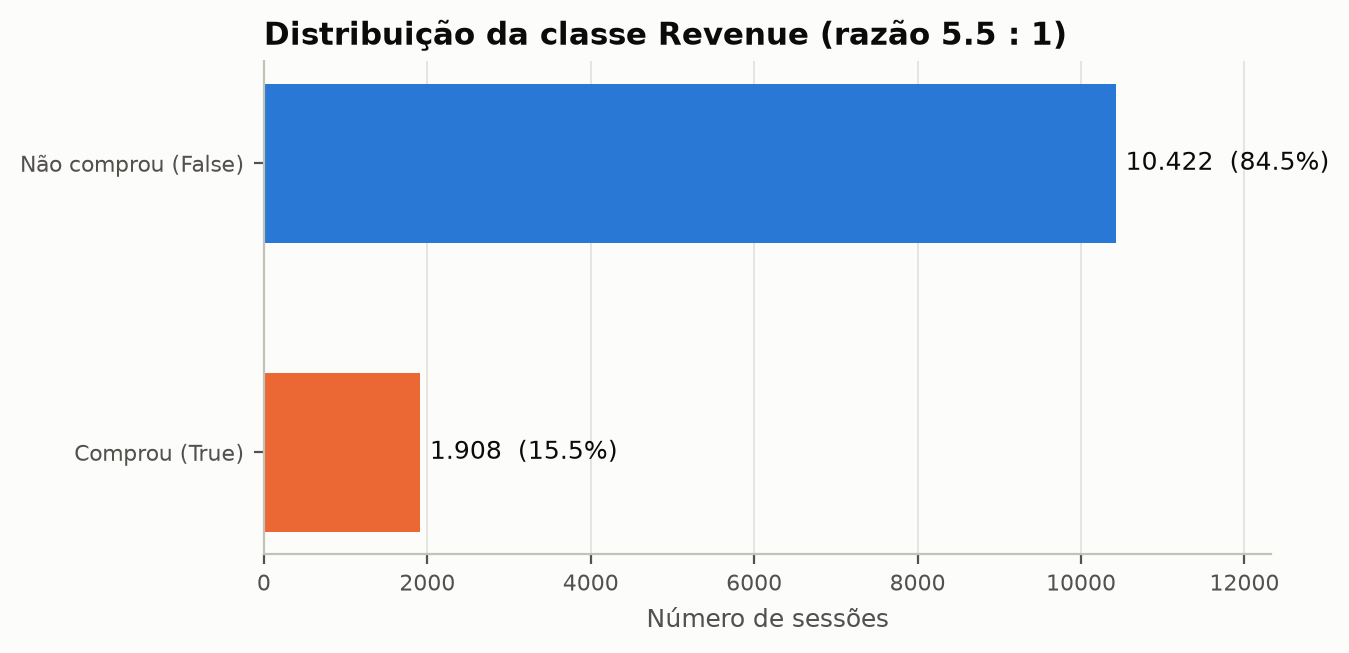
\includegraphics[width=0.78\textwidth]{01_distribuicao_classes.png}
  \caption{Distribuição da classe \atr{Revenue}.}
  \label{fig:classes}
\end{figure}

\begin{figure}[H]
  \centering
  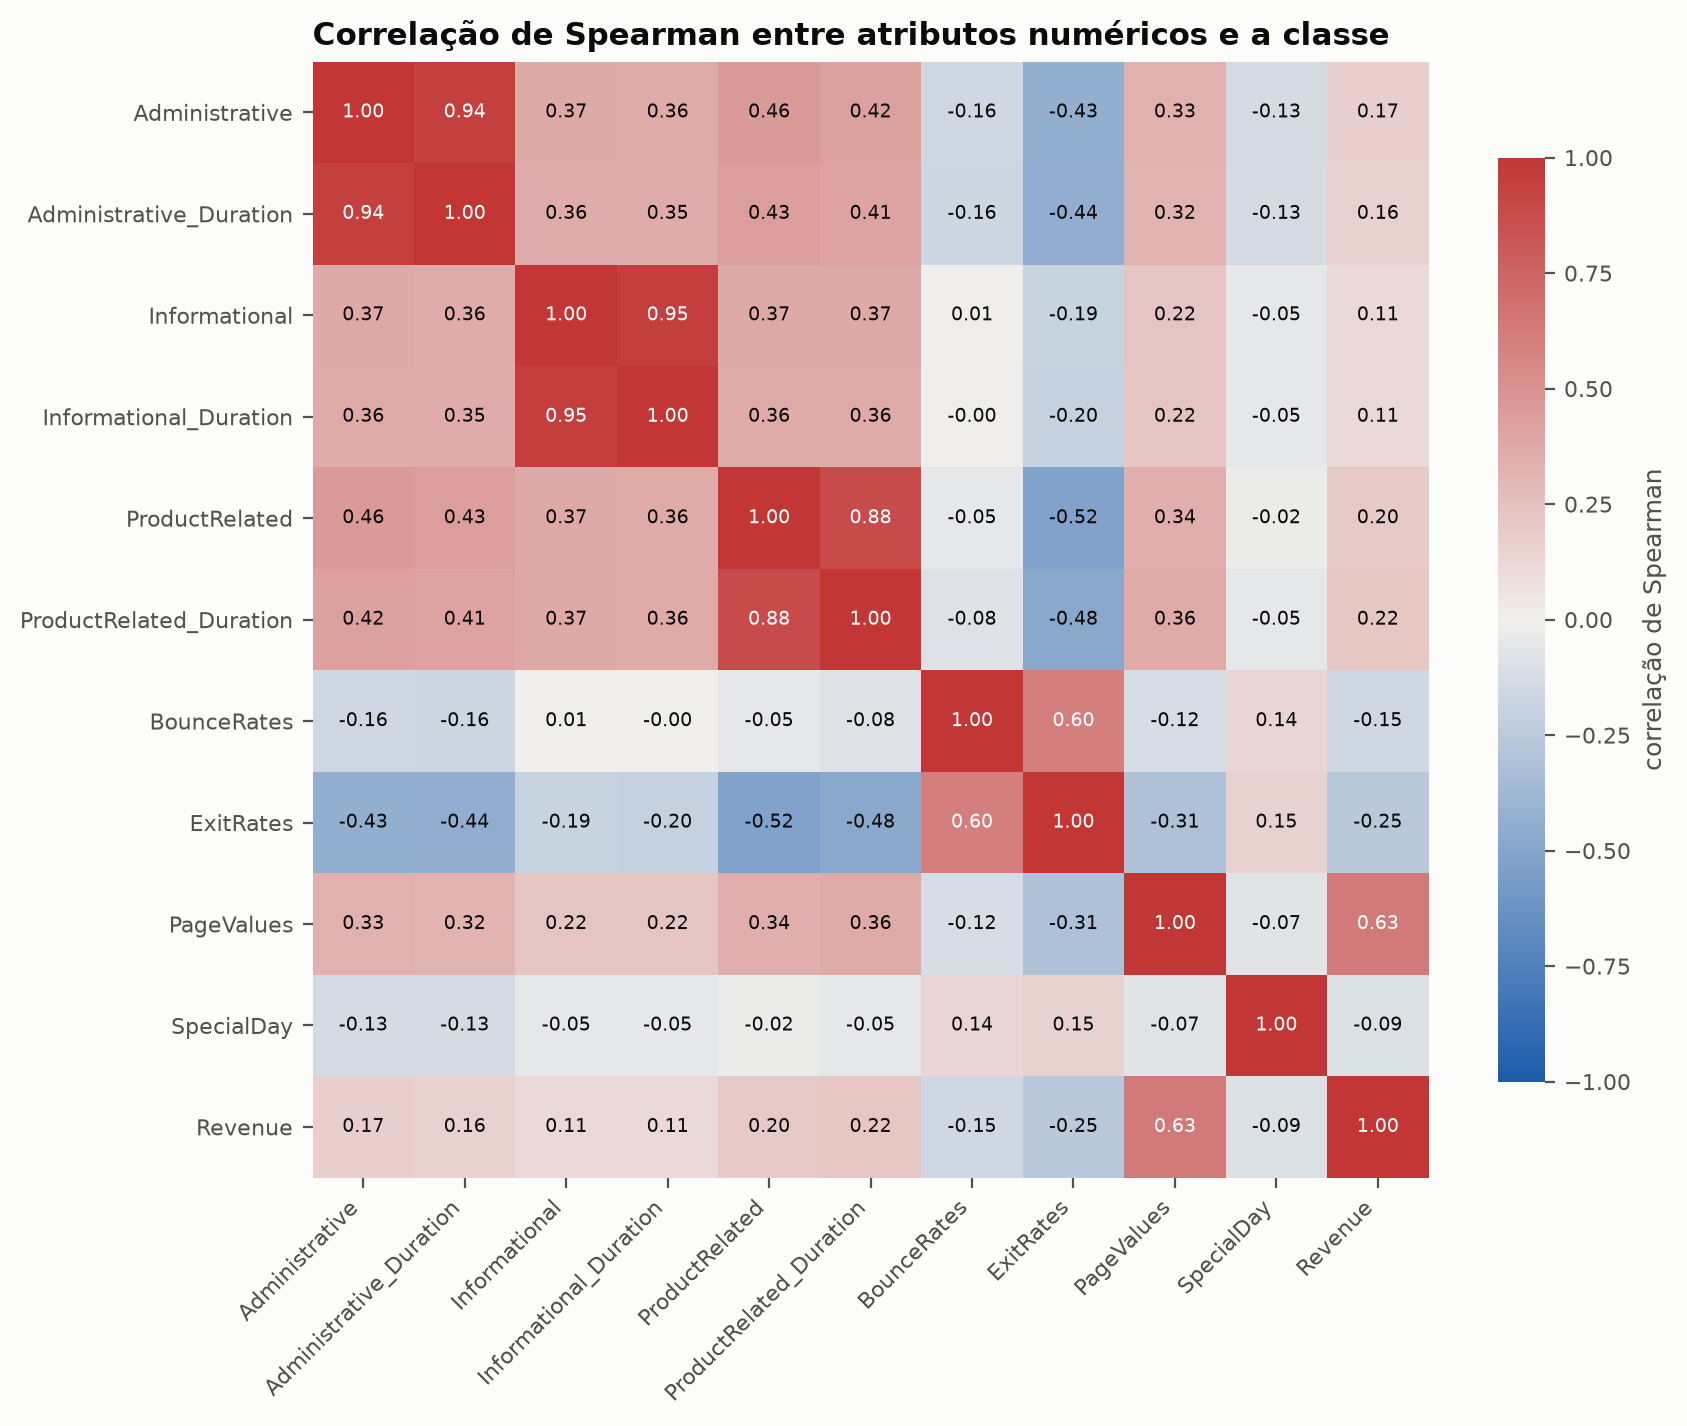
\includegraphics[width=0.9\textwidth]{05_correlacao_spearman.png}
  \caption{Correlação de Spearman entre os atributos numéricos e a classe.}
  \label{fig:correlacao}
\end{figure}

\begin{figure}[H]
  \centering
  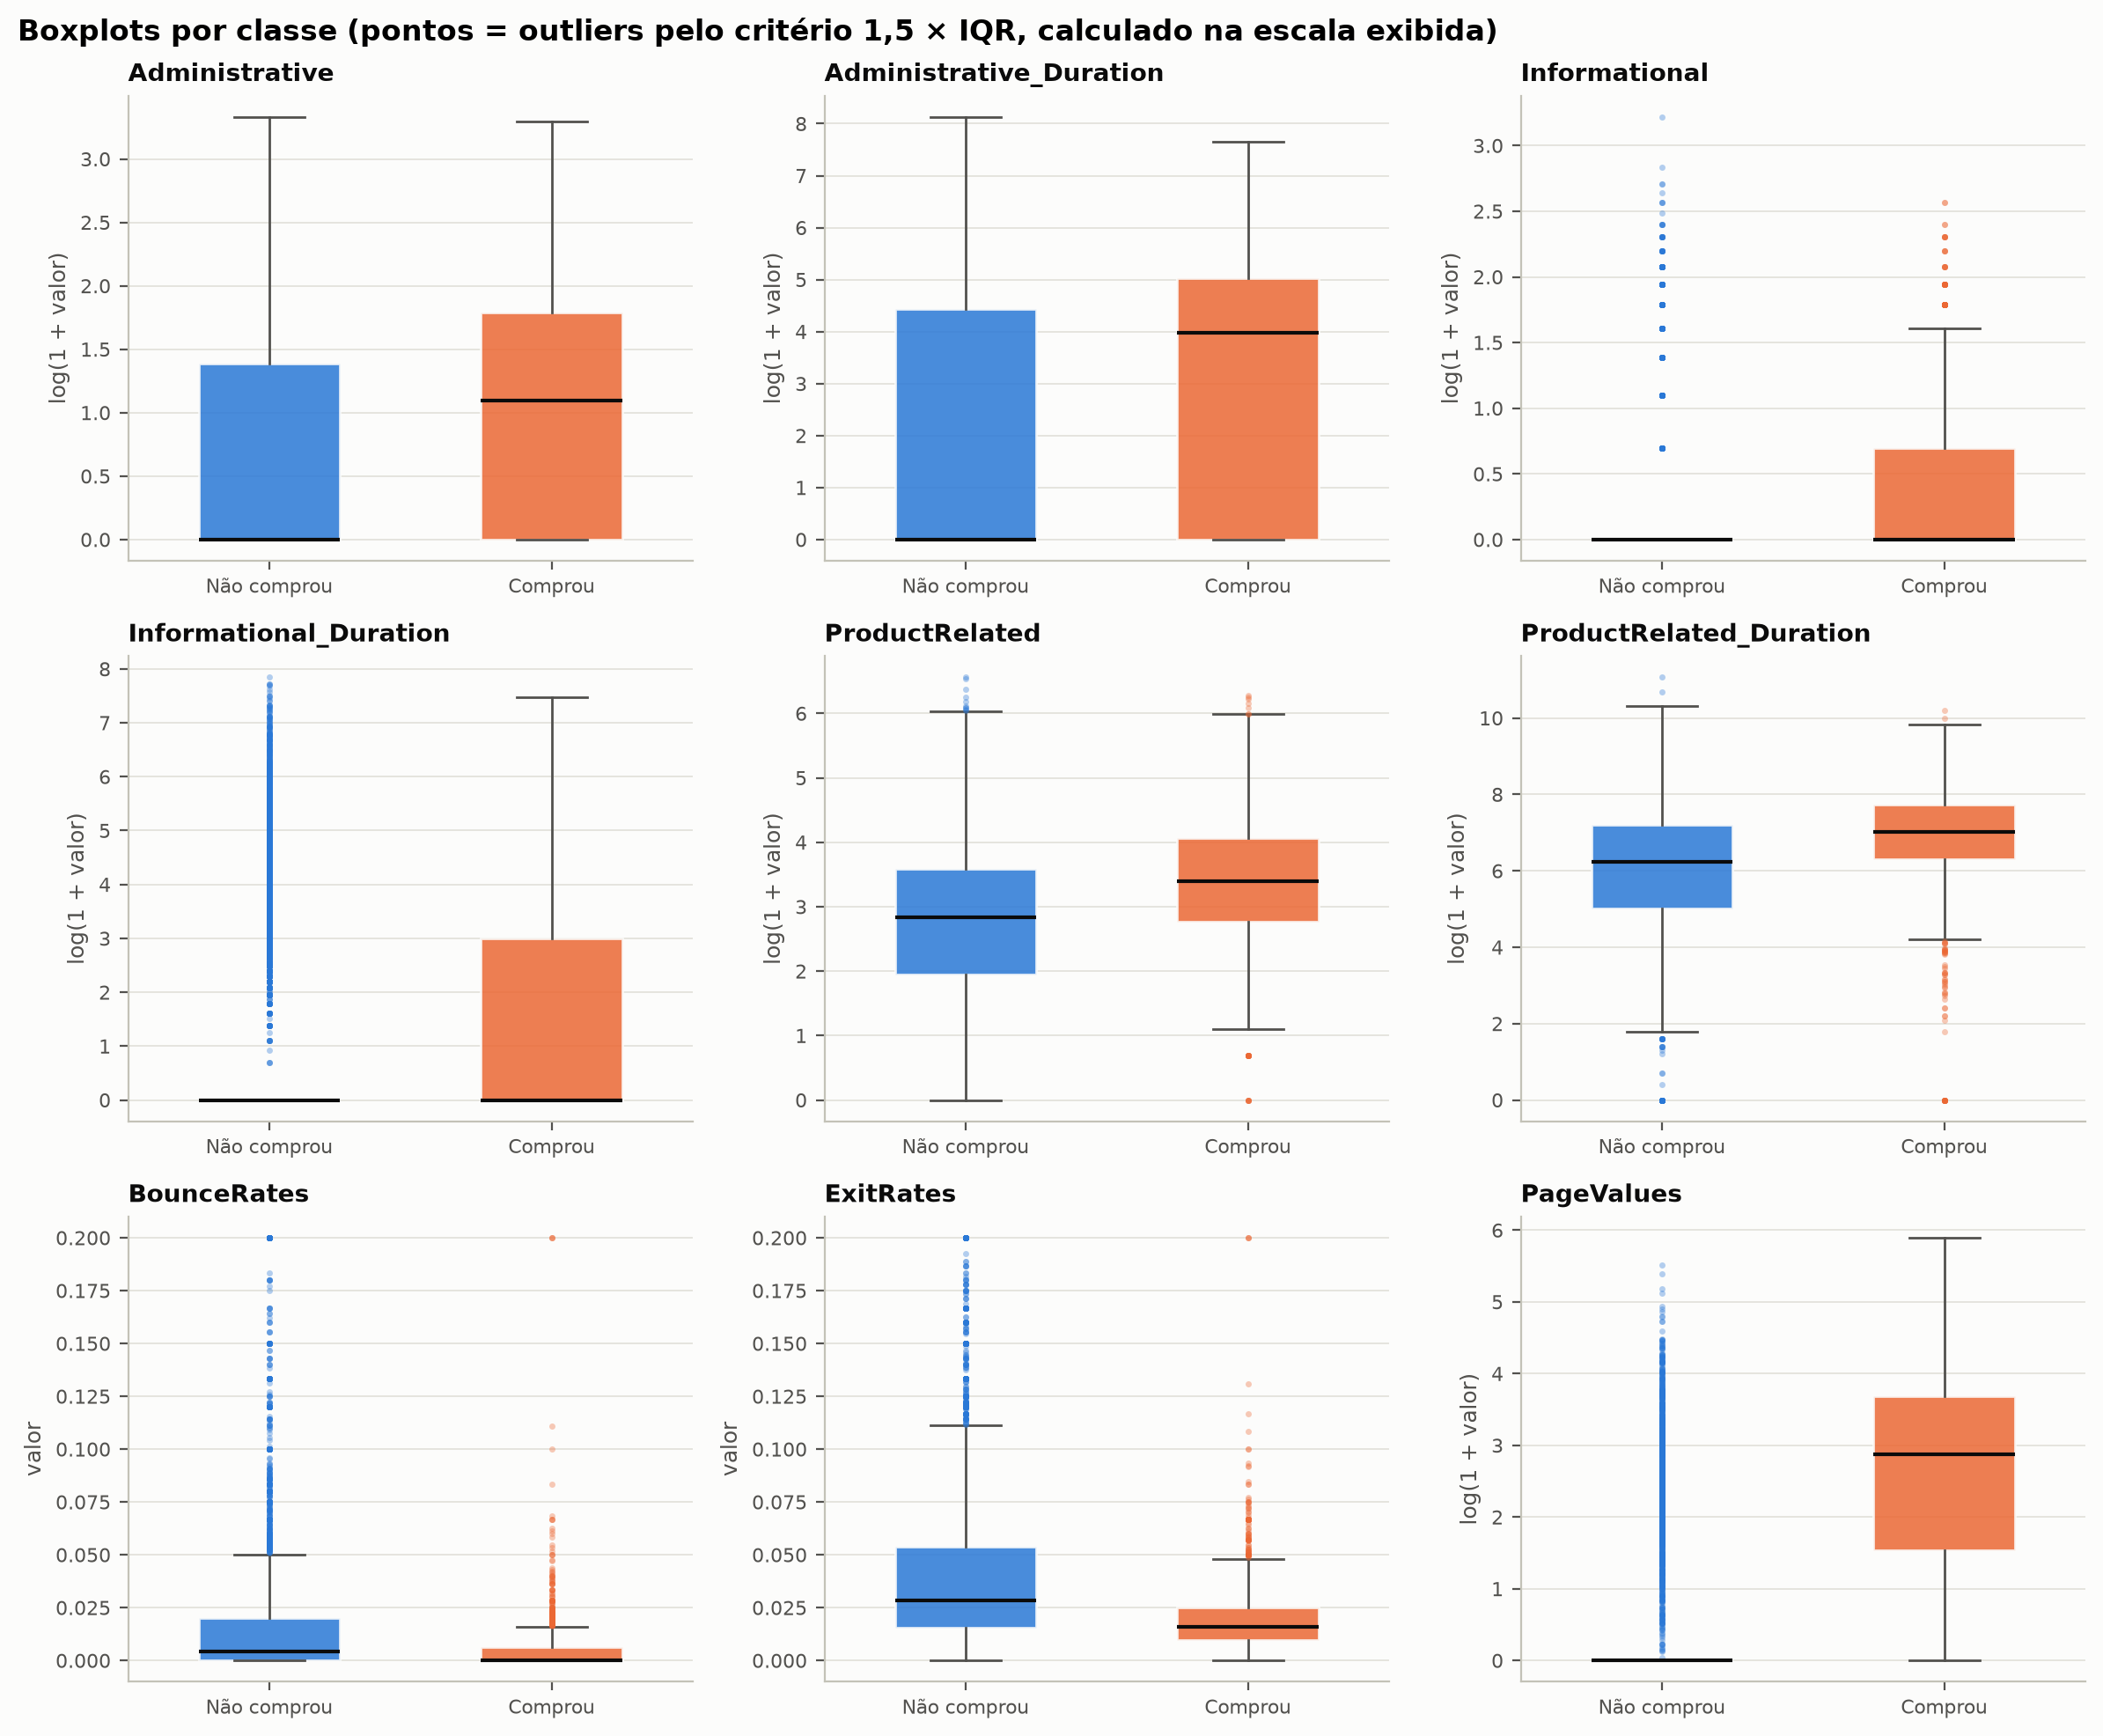
\includegraphics[width=\textwidth]{03_boxplots_por_classe.png}
  \caption{Boxplots dos atributos numéricos por classe, em escala $\log(1+x)$ para os atributos assimétricos. Os
           pontos são outliers pelo critério de 1,5\,$\times$\,IQR.}
  \label{fig:boxplots}
\end{figure}

% ============================================================================= III
\section{Metodologia}

\subsection{Pré-processamento e justificativas}

\begin{itemize}
  \item \textbf{Remover duplicatas para todos os algoritmos.} Com base na análise exploratória, verificamos que
        alguns registros estão duplicados. Devemos fazer sua remoção principalmente porque vamos usar o k-fold cross
        validation: uma cópia poderia cair no treino e outra no teste.
  \item \textbf{Padronizar e converter tipos, em todos os algoritmos.} O mês \atr{June} foi padronizado para
        \atr{Jun}, e \atr{Weekend} e \atr{Revenue} foram convertidos de True/False para 1/0. Junto com a remoção de
        duplicatas, essas etapas não aprendem nada com os dados e por isso foram aplicadas uma única vez, antes da
        divisão em treino e teste. A base resultante tem 12.205 sessões, das quais 15,63\% terminam em compra.
  \item \textbf{Manter os outliers em todos os algoritmos.} As sessões com valores extremos compram mais que a média
        (23\% a 30\%, contra 15,5\%), ou seja, os valores extremos são informativos e não erros.
  \item \textbf{Remover dimensões para os algoritmos KNN e MLP.} Com base no gráfico de correlações, verificamos uma
        correlação clara ($\rho$ de 0,88 a 0,95) entre os pares:
        \begin{itemize}
          \item \atr{Administrative} e \atr{Administrative\_Duration};
          \item \atr{Informational} e \atr{Informational\_Duration};
          \item \atr{ProductRelated} e \atr{ProductRelated\_Duration}.
        \end{itemize}
        Em cada par foi removida a contagem e mantida a duração, que carrega a mesma informação com mais
        detalhe. No Random Forest e no Gradient Boosting todos os atributos foram mantidos, porque a correlação entre
        atributos não prejudica a predição das árvores.
  \item \textbf{Usar $\log(1+x)$ e min-max no KNN}, para os atributos ficarem na mesma escala. O $\log(1+x)$ é
        aplicado antes do min-max nas durações e em \atr{PageValues}, que são muito assimétricos: sem o log, os
        poucos valores extremos definiriam o máximo do min-max e a maioria das sessões ficaria comprimida perto de 0,
        sem diferença entre elas no cálculo da distância. As taxas (\atr{BounceRates}, \atr{ExitRates} e
        \atr{SpecialDay}) já estão entre 0 e 1 e recebem só o min-max.
  \item \textbf{Usar padronização (z-score) no MLP}, para os atributos numéricos ficarem centrados (média) em 0 e com
        desvio padrão 1. A rede aprende por gradiente, e entradas em escalas muito diferentes deixam o treino instável
        e lento: por exemplo, \atr{ProductRelated\_Duration} chega a 63.973, enquanto \atr{ExitRates} não passa de
        0,2.
  \item \textbf{Usar one-hot encoding no KNN e no MLP} para converter os atributos categóricos em numéricos, já que
        esses algoritmos fazem cálculos (distâncias e somas ponderadas) que só lidam com números.
  \item \textbf{Agrupar categorias raras no KNN e no MLP}, com o objetivo de reduzir o ruído. Foram consideradas
        raras as categorias presentes em menos de 1\% das sessões de treino: os sistemas operacionais 5 a 8; os
        navegadores 3, 7, 9, 11, 12 e 13; os tipos de tráfego 7, 9, 12, 14, 15, 16, 18 e 19; e o tipo de visitante
        \textit{Other}. Cada atributo ganha uma única coluna para as suas categorias raras. Após o one-hot, o KNN e o
        MLP recebem 55 colunas: 47 vindas dos atributos categóricos, 7 numéricas e \atr{Weekend}.
  \item \textbf{Manter os atributos categóricos como códigos inteiros no Random Forest.} \atr{OperatingSystems},
        \atr{Browser}, \atr{Region} e \atr{TrafficType} já são inteiros; \atr{Month} e \atr{VisitorType} precisam ser
        convertidos em códigos. As árvores dividem os dados por limiares e não calculam distâncias, então os códigos
        funcionam e ainda permitem separar grupos de categorias. Com one-hot, o \atr{TrafficType} viraria 20 colunas
        binárias, cada uma raramente escolhida para divisão.
  \item \textbf{Usar os atributos categóricos de forma nativa no Gradient Boosting.} O
        \atr{HistGradientBoostingClassifier} do scikit-learn aceita atributos categóricos diretamente: em cada
        divisão, ele separa as categorias em dois grupos, sem precisar de one-hot e sem impor uma ordem artificial aos
        códigos.
  \item \textbf{Tratar o desbalanceamento em todos os algoritmos.} Com base na análise exploratória, 84,5\% das
        sessões são ``não comprou'' e 15,5\% são ``comprou''. Sem tratamento, os algoritmos tendem a favorecer a
        classe majoritária.
        \begin{itemize}
          \item \textbf{KNN:} sobreamostragem da classe minoritária, aplicada só nos folds de treino do k-fold. O KNN
                não aceita pesos por classe, e com 84,5\% de ``não comprou'' os vizinhos mais próximos tendem a ser
                dessa classe. Foi usada a sobreamostragem aleatória (\atr{RandomOverSampler}), que repete sessões da
                classe minoritária até as duas classes ficarem com o mesmo tamanho. O SMOTE comum foi descartado
                porque interpolaria as colunas one-hot e criaria valores sem sentido, como 0,4; o SMOTENC, que trata
                atributos categóricos, fica como possível melhoria.
          \item \textbf{Random Forest:} \atr{class\_weight="balanced"}, que dá a cada classe um peso inversamente
                proporcional à sua frequência. Assim, errar uma sessão ``comprou'' pesa cerca de 5,4 vezes mais, sem
                alterar os dados.
          \item \textbf{Gradient Boosting:} \atr{class\_weight="balanced"}, pelo mesmo motivo do Random Forest.
          \item \textbf{MLP:} sobreamostragem da classe minoritária, aplicada só nos folds de treino, já que o
                \atr{MLPClassifier} do scikit-learn não aceita pesos por classe.
        \end{itemize}
  \item \textbf{Evitar vazamento de informação.} Todas as etapas que aprendem algo com os dados (min-max, z-score,
        agrupamento de categorias raras e sobreamostragem) foram montadas em um \atr{Pipeline} da biblioteca
        imbalanced-learn e são ajustadas somente na parte de treino de cada fold da validação cruzada. A parte de
        avaliação nunca é sobreamostrada e mantém a proporção real das classes.
\end{itemize}

A Tabela~\ref{tab:preproc} resume o pré-processamento aplicado em cada algoritmo.

\begin{table}[H]
  \centering\small
  \caption{Pré-processamento por algoritmo.}
  \label{tab:preproc}
  \begin{tabularx}{\textwidth}{Ycccc}
    \toprule
    Etapa & KNN & Random Forest & Gradient Boosting & MLP\\
    \midrule
    Remover duplicatas, June $\to$ Jun, booleanos $\to$ 0/1 & sim & sim & sim & sim\\
    Remover contagens redundantes & sim & não & não & sim\\
    $\log(1+x)$ & sim & não & não & não\\
    Escala & min-max & não & não & z-score\\
    Atributos categóricos & one-hot & códigos inteiros & categóricos nativos & one-hot\\
    Agrupar categorias raras & sim & não & não & sim\\
    Desbalanceamento & sobreamostragem & \atr{class\_weight} & \atr{class\_weight} & sobreamostragem\\
    \bottomrule
  \end{tabularx}
\end{table}

\subsection{Ferramentas}

Todo o trabalho foi feito em Python 3.13, em notebooks Jupyter, dentro de um ambiente virtual gerenciado pelo uv, que
fixa as versões das bibliotecas e permite reproduzir os resultados. O código foi organizado em três notebooks, um por
fase: análise exploratória, pré-processamento e classificação. As bibliotecas usadas foram:
\begin{itemize}
  \item \textbf{pandas} 3.1.1 e \textbf{NumPy} 2.5.4: leitura e manipulação dos dados;
  \item \textbf{Matplotlib} 3.11.2: gráficos;
  \item \textbf{scikit-learn} 1.9.1: algoritmos de classificação, transformações (min-max, z-score, one-hot, códigos
        inteiros), pipelines, validação cruzada, busca em grade e medidas de avaliação;
  \item \textbf{imbalanced-learn} 0.14.2: sobreamostragem aleatória (\atr{RandomOverSampler}) e o \atr{Pipeline}
        que aplica a sobreamostragem apenas nos dados de treino.
\end{itemize}
Em todos os passos aleatórios (divisão dos dados, folds, sobreamostragem e inicialização dos modelos) foi usada a
semente 42.

\subsection{Algoritmos de classificação}

Foram usados quatro algoritmos. Os
parâmetros testados para cada algoritmo estão na Tabela~\ref{tab:grade}.

\subsubsection*{1) KNN (k vizinhos mais próximos)}

\textbf{Funcionamento.} O KNN não constrói um modelo durante o treino: ele apenas guarda as sessões de treino. Para
classificar uma sessão nova, calcula a distância dela até todas as sessões de treino, seleciona as $k$ mais próximas
e atribui a classe mais votada entre elas. O voto pode ser uniforme ou ponderado pelo inverso da distância, e a
probabilidade de compra é a fração (ponderada) de vizinhos compradores. A distância usada é a de Minkowski, que com
$p = 1$ é a distância de Manhattan e com $p = 2$ é a euclidiana. Os dois valores de $p$ foram testados na busca em
grade (Tabela~\ref{tab:grade}), e o modelo final usa a distância de Manhattan ($p = 1$), que obteve F1 maior que a
euclidiana em todos os valores de $k$ testados (Seção~\ref{sec:resultados_grade}).

\textbf{Justificativa.} É um classificador simples, não paramétrico e sem suposições sobre a forma da fronteira de
decisão, o que o torna uma boa referência. Como depende de distâncias, também mostra o efeito do pré-processamento
(escala, assimetria e codificação dos atributos categóricos) sobre o resultado.

\textbf{Parâmetros.} O número de vizinhos $k$ controla o equilíbrio entre um modelo que segue o ruído ($k$ pequeno) e
um modelo que suaviza demais a fronteira ($k$ grande). O tipo de peso e a distância mudam quanto cada vizinho e cada
atributo influenciam a decisão.

\textbf{Pré-processamento necessário.} Remoção das contagens redundantes, $\log(1+x)$ e min-max nos atributos
numéricos, one-hot com agrupamento de categorias raras e sobreamostragem. O KNN exige atributos numéricos e na mesma
escala, pois um atributo com valores grandes dominaria a distância.

\subsubsection*{2) Random Forest }

\textbf{Funcionamento.} O Random Forest (Breiman, 2001) é um conjunto (\textit{ensemble}) de árvores de decisão cujas
previsões são combinadas por votação. Uma árvore de decisão divide as sessões de forma recursiva: em cada nó, escolhe
um atributo e um limiar (por exemplo, $\texttt{PageValues} \le 0{,}5$) que separam as sessões em dois grupos mais
homogêneos quanto à classe, e repete o processo em cada grupo até atingir um critério de parada. A homogeneidade é
medida pela impureza de Gini,
\begin{equation*}
  \mathrm{Gini}(D) = 1 - p_1^2 - p_0^2,
\end{equation*}
em que $p_1$ e $p_0$ são as proporções de sessões com e sem compra no grupo $D$. A melhor divisão é a que mais reduz
a impureza média dos dois grupos resultantes, e cada folha guarda a proporção de compradores das sessões que caíram
nela.

Uma única árvore profunda decora o treino e varia muito com pequenas mudanças nos dados. O Random Forest reduz essa
variância com duas fontes de aleatoriedade: (1) cada árvore é treinada com uma amostra \textit{bootstrap}, isto é,
$n$ sessões sorteadas com reposição do treino; e (2) em cada nó, a melhor divisão é procurada apenas entre $m$
atributos sorteados (\atr{max\_features}), e não entre todos. Assim, as árvores ficam diferentes entre si e seus erros
se compensam. A probabilidade de compra prevista é a média das probabilidades dadas por todas as árvores, e a sessão é
classificada como compra se essa média for pelo menos 0,5.

Com \atr{class\_weight="balanced"}, cada sessão recebe um peso inversamente proporcional à frequência da sua classe
(cerca de 3,2 para as sessões com compra e 0,59 para as demais). Os pesos entram no cálculo da impureza de Gini e das
proporções nas folhas, de modo que errar uma sessão com compra pesa cerca de 5,4 vezes mais. O pseudocódigo está no
Algoritmo~\ref{alg:rf}.

\begin{algorithm}[H]
  \caption{Random Forest para classificação binária}
  \label{alg:rf}
  \small
  \begin{algorithmic}[1]
    \Require treino $D = \{(x_i, y_i)\}_{i=1}^{n}$ com pesos por classe $w_i$; número de árvores $B$
             (\atr{n\_estimators}); atributos por divisão $m$ (\atr{max\_features}); \atr{max\_depth};
             \atr{min\_samples\_leaf}
    \For{$b = 1$ \textbf{até} $B$}
      \State $D_b \gets$ $n$ sessões sorteadas com reposição de $D$ \Comment{amostra bootstrap}
      \State $T_b \gets \Call{ConstruirÁrvore}{D_b, 0}$
    \EndFor
    \Ensure $P(\text{comprou} \mid x) = \frac{1}{B}\sum_{b=1}^{B} P_b(\text{comprou} \mid x)$; classe = comprou se
            $P \ge 0{,}5$
    \Statex
    \Function{ConstruirÁrvore}{$D$, $prof$}
      \If{$D$ tem uma só classe \textbf{ou} $prof = \texttt{max\_depth}$ \textbf{ou}
          $|D| < 2 \cdot \texttt{min\_samples\_leaf}$}
        \State \Return folha com $P(\text{comprou}) =$ peso dos compradores em $D$ / peso total de $D$
      \EndIf
      \State $A \gets$ $m$ atributos sorteados sem reposição
      \ForAll{atributo $a \in A$ e limiar $t$ entre valores consecutivos de $a$ em $D$}
        \State $D_E \gets \{x \in D : x_a \le t\}$; \quad $D_D \gets D \setminus D_E$
        \State $\Delta(a,t) \gets \mathrm{Gini}(D) - \frac{|D_E|}{|D|}\mathrm{Gini}(D_E) -
               \frac{|D_D|}{|D|}\mathrm{Gini}(D_D)$ \Comment{tamanhos ponderados por $w_i$}
      \EndFor
      \State $(a^*, t^*) \gets \arg\max \Delta(a,t)$
      \State $T_E \gets \Call{ConstruirÁrvore}{D_E, prof+1}$; \quad $T_D \gets \Call{ConstruirÁrvore}{D_D, prof+1}$
      \State \Return nó com o teste $x_{a^*} \le t^*$, filho esquerdo $T_E$ e filho direito $T_D$
    \EndFunction
  \end{algorithmic}
\end{algorithm}

\textbf{Justificativa.} Lida bem com atributos de tipos diferentes, com relações não lineares e com interações entre
atributos, não exige normalização e não é afetado pela assimetria nem pelos outliers, pois as árvores dividem os dados
por limiares. Também aceita pesos por classe para tratar o desbalanceamento e é pouco propenso a sobreajuste, por
fazer a média de muitas árvores.

\textbf{Parâmetros.} O número de árvores, a quantidade de atributos sorteados em cada divisão, a profundidade máxima e
o mínimo de instâncias por folha. Os dois últimos limitam o quanto cada árvore pode decorar o treino.

\textbf{Pré-processamento necessário.} Apenas a conversão de \atr{Month} e \atr{VisitorType} em códigos inteiros. Os
demais atributos são usados como estão, e o desbalanceamento é tratado com \atr{class\_weight="balanced"}.

\subsubsection*{3) Gradient Boosting}

\textbf{Funcionamento.} O Gradient Boosting (Friedman, 2001) também combina árvores de decisão, mas de forma
sequencial: cada nova árvore é treinada para corrigir os erros do conjunto formado pelas árvores anteriores. O modelo
é uma soma
\begin{equation*}
  F(x) = F_0 + \eta\,T_1(x) + \eta\,T_2(x) + \dots + \eta\,T_M(x),
\end{equation*}
em que cada $T_m$ é uma árvore de regressão pequena e $\eta$ é a taxa de aprendizado. Para classificação binária,
$F(x)$ é o logaritmo da razão de chances de compra, e a probabilidade é obtida pela função sigmoide,
$P(\text{comprou} \mid x) = 1 / (1 + e^{-F(x)})$.

Em cada iteração, o algoritmo calcula, para cada sessão de treino, o gradiente da perda logística em relação à
previsão atual ($g = p - y$, a diferença entre a probabilidade prevista e a classe real) e a curvatura dessa perda
($h = p(1-p)$). A nova árvore é construída para seguir a direção oposta ao gradiente, ou seja, para reduzir a perda
onde o modelo mais erra. A taxa de aprendizado $\eta$ reduz o tamanho de cada passo, o que torna o modelo mais
estável e menos propenso a sobreajuste, mas exige mais árvores.

A implementação usada foi o \atr{HistGradientBoostingClassifier} do scikit-learn, inspirado no LightGBM (Ke et al.,
2017). Ele discretiza cada atributo numérico em no máximo 255 faixas (histogramas), o que torna a busca da melhor
divisão muito mais rápida, e trata atributos categóricos de forma nativa, separando as categorias em dois grupos a
cada divisão. Os pesos por classe (\atr{class\_weight}) multiplicam o gradiente e a curvatura de cada sessão, de modo
que os erros nas sessões com compra pesam mais. O pseudocódigo está no Algoritmo~\ref{alg:gb}.

\begin{algorithm}[H]
  \caption{Gradient Boosting com histogramas para classificação binária}
  \label{alg:gb}
  \small
  \begin{algorithmic}[1]
    \Require treino $\{(x_i, y_i)\}_{i=1}^{n}$, $y_i \in \{0,1\}$, com pesos por classe $w_i$; número de árvores $M$
             (\atr{max\_iter}); taxa de aprendizado $\eta$; limites da árvore (\atr{max\_depth}, máximo de 31
             folhas); regularização $\lambda$
    \State discretizar cada atributo numérico em até 255 faixas (histogramas)
    \State $p \gets$ proporção ponderada de compradores no treino
    \State $F_0(x) \gets \log\big(p / (1-p)\big)$ \Comment{previsão inicial igual para todos}
    \For{$m = 1$ \textbf{até} $M$}
      \ForAll{sessão $i$}
        \State $p_i \gets 1 / \big(1 + e^{-F_{m-1}(x_i)}\big)$ \Comment{probabilidade atual}
        \State $g_i \gets w_i\,(p_i - y_i)$ \Comment{gradiente da perda logística}
        \State $h_i \gets w_i\,p_i\,(1 - p_i)$ \Comment{curvatura (2ª derivada)}
      \EndFor
      \State $T_m \gets$ nova árvore com todas as sessões na raiz
      \While{houver folha que possa ser dividida respeitando os limites}
        \ForAll{atributo e fronteira entre faixas (ou grupo de categorias)}
          \State $G_E, H_E \gets$ somas de $g$ e $h$ à esquerda; \quad $G_D, H_D \gets$ somas à direita
          \State $\text{ganho} \gets \frac{G_E^2}{H_E+\lambda} + \frac{G_D^2}{H_D+\lambda} -
                 \frac{(G_E+G_D)^2}{H_E+H_D+\lambda}$
        \EndFor
        \State dividir a folha pela fronteira de maior ganho
      \EndWhile
      \ForAll{folha $j$ de $T_m$}
        \State $v_j \gets -\sum_{i \in j} g_i \,/\, \big(\sum_{i \in j} h_i + \lambda\big)$
      \EndFor
      \State $F_m(x) \gets F_{m-1}(x) + \eta\,T_m(x)$ \Comment{$T_m(x)$ = valor da folha em que $x$ cai}
    \EndFor
    \Ensure $P(\text{comprou} \mid x) = 1/\big(1 + e^{-F_M(x)}\big)$; classe = comprou se $P \ge 0{,}5$
  \end{algorithmic}
\end{algorithm}

\textbf{Justificativa.} O Gradient Boosting está entre os algoritmos com melhor desempenho em dados tabulares.
Enquanto o Random Forest reduz a variância fazendo a média de árvores independentes, o boosting reduz o viés
corrigindo erros de forma sequencial, o que permite comparar as duas estratégias de combinação de árvores. Assim como
o Random Forest, não exige normalização e não é afetado pela assimetria dos atributos.

\textbf{Parâmetros.} A taxa de aprendizado $\eta$, o número de árvores $M$ e a profundidade máxima de cada árvore.
Taxas maiores com muitas árvores tendem a sobreajustar; taxas menores precisam de mais árvores.

\textbf{Pré-processamento necessário.} Apenas a conversão dos atributos categóricos em códigos para o tratamento
nativo. O desbalanceamento é tratado com \atr{class\_weight="balanced"}.

\subsubsection*{4) Rede neural MLP -- Multilayer Perceptron}

\textbf{Funcionamento.} O MLP é uma rede neural formada por camadas de neurônios totalmente conectadas. Neste trabalho
a rede tem três camadas: a de entrada, com uma posição para cada uma das 55 colunas produzidas pelo
pré-processamento; uma camada oculta com $H$ neurônios; e a de saída, com um único neurônio. Cada neurônio oculto
calcula uma soma ponderada das entradas, soma um viés e aplica uma função de ativação não linear $\varphi$ (ReLU,
$\varphi(z) = \max(0, z)$, ou tangente hiperbólica). O neurônio de saída faz o mesmo com as saídas da camada oculta e
aplica a sigmoide, produzindo a probabilidade de compra. É a camada oculta não linear que permite à rede aprender
fronteiras de decisão complexas.

O treino ajusta os pesos para minimizar a perda logística (entropia cruzada) somada a uma penalidade L2,
$\alpha\lVert W\rVert^2$, que desestimula pesos grandes e reduz o sobreajuste. O gradiente da perda em relação a cada
peso é calculado pela retropropagação (Rumelhart, Hinton e Williams, 1986), que aplica a regra da cadeia da saída para
a entrada. Os pesos são atualizados pelo otimizador Adam (Kingma e Ba, 2015) em lotes de 200 sessões, e o treino para
quando a perda deixa de melhorar por 10 épocas seguidas ou ao atingir o limite de épocas. O pseudocódigo está no
Algoritmo~\ref{alg:mlp}.

\begin{algorithm}[H]
  \caption{Treino do MLP com uma camada oculta}
  \label{alg:mlp}
  \small
  \begin{algorithmic}[1]
    \Require treino padronizado e balanceado $\{(x_i, y_i)\}_{i=1}^{n}$, $x_i \in \mathbb{R}^{55}$; $H$ neurônios
             ocultos; ativação $\varphi$ (ReLU ou tanh); regularização $\alpha$; taxa $\eta = 0{,}001$; lote
             $B = 200$; limite de 1000 épocas
    \State inicializar $W_1 \in \mathbb{R}^{55 \times H}$, $b_1$, $W_2 \in \mathbb{R}^{H \times 1}$, $b_2$ com
           valores aleatórios pequenos
    \For{época $= 1$ \textbf{até} $1000$}
      \State embaralhar o treino e dividi-lo em lotes de $B$ sessões
      \ForAll{lote $(X, y)$}
        \State $A \gets \varphi(X W_1 + b_1)$ \Comment{camada oculta}
        \State $\hat{y} \gets 1 / \big(1 + e^{-(A W_2 + b_2)}\big)$ \Comment{probabilidade de compra}
        \State $L \gets -\operatorname{média}\big[y \log \hat{y} + (1-y)\log(1-\hat{y})\big] +
               \frac{\alpha}{2n}\big(\lVert W_1\rVert^2 + \lVert W_2\rVert^2\big)$
        \State $\delta_2 \gets \hat{y} - y$ \Comment{erro na saída}
        \State $\nabla W_2 \gets A^{\top}\delta_2 / B + \frac{\alpha}{n} W_2$; \quad
               $\nabla b_2 \gets \operatorname{média}(\delta_2)$
        \State $\delta_1 \gets (\delta_2 W_2^{\top}) \odot \varphi'(X W_1 + b_1)$ \Comment{erro retropropagado}
        \State $\nabla W_1 \gets X^{\top}\delta_1 / B + \frac{\alpha}{n} W_1$; \quad
               $\nabla b_1 \gets \operatorname{média}(\delta_1)$
        \State atualizar $W_1, b_1, W_2, b_2$ com o Adam usando os gradientes
      \EndFor
      \If{a perda não melhorar mais que $10^{-4}$ por 10 épocas seguidas}
        \State parar
      \EndIf
    \EndFor
    \Ensure $P(\text{comprou} \mid x) = \hat{y}(x)$; classe = comprou se $P \ge 0{,}5$
  \end{algorithmic}
\end{algorithm}

\textbf{Justificativa.} As redes neurais conseguem aproximar relações não lineares complexas e são uma abordagem
diferente das árvores, o que enriquece a comparação. Além disso, o artigo que publicou esta base (Sakar et al., 2019)
usou justamente um MLP para prever a intenção de compra.

\textbf{Parâmetros.} O número de neurônios da camada oculta (capacidade da rede), a força da regularização $\alpha$ e
a função de ativação. Com poucos dados e muitos parâmetros, a regularização é o que impede a rede de decorar o treino.

\textbf{Pré-processamento necessário.} Remoção das contagens redundantes, z-score nos atributos numéricos, one-hot com
agrupamento de categorias raras e sobreamostragem. A rede aprende por gradiente, e atributos em escalas muito
diferentes deixariam o treino instável e lento.

\subsection{Parâmetros testados}

Os parâmetros não foram fixados previamente. Para cada algoritmo, os principais parâmetros receberam uma lista de
valores, e todas as combinações foram avaliadas por busca em grade (\atr{GridSearchCV}), totalizando 72 combinações
(Tabela~\ref{tab:grade}). Os valores cobrem desde modelos mais simples até modelos mais complexos, para mostrar como
cada parâmetro afeta o resultado.

\begin{table}[H]
  \centering\footnotesize
  \caption{Grade de parâmetros testada em cada algoritmo.}
  \label{tab:grade}
  \begin{tabularx}{\textwidth}{@{}lllY@{}}
    \toprule
    Algoritmo & Parâmetro & Valores testados & O que controla\\
    \midrule
    KNN & \atr{n\_neighbors} & 5, 15, 31, 51, 101 & Número de vizinhos que votam\\
    (20 combinações) & \atr{weights} & uniform, distance & Voto igual ou ponderado pela distância\\
     & \atr{p} & 1 (Manhattan), 2 (euclidiana) & Distância usada\\
    \midrule
    Random Forest & \atr{n\_estimators} & 100, 300 & Número de árvores\\
    (16 combinações) & \atr{max\_features} & sqrt, 0,5 & Atributos sorteados em cada divisão\\
     & \atr{max\_depth} & sem limite, 10 & Profundidade máxima das árvores\\
     & \atr{min\_samples\_leaf} & 1, 5 & Mínimo de instâncias por folha\\
    \midrule
    Gradient Boosting & \atr{learning\_rate} & 0,05; 0,1; 0,2 & Tamanho do passo de cada árvore\\
    (18 combinações) & \atr{max\_iter} & 100, 300 & Número de árvores\\
     & \atr{max\_depth} & sem limite, 3, 6 & Profundidade de cada árvore\\
    \midrule
    MLP & \atr{hidden\_layer\_sizes} & 10, 50, 100 neurônios & Tamanho da camada oculta\\
    (18 combinações) & \atr{alpha} & 0,0001; 0,01; 1 & Força da regularização L2\\
     & \atr{activation} & relu, tanh & Função de ativação\\
    \bottomrule
  \end{tabularx}
\end{table}

Alguns valores foram mantidos fixos: a semente aleatória (42), para tornar os resultados reprodutíveis; o tratamento
do desbalanceamento (\atr{class\_weight} ou sobreamostragem), que faz parte do pré-processamento; e o limite de 1000
épocas do MLP, que é um critério de parada e não um parâmetro do modelo, já que o treino para antes quando a perda
deixa de melhorar. Os demais parâmetros usam os valores padrão do scikit-learn.

\subsection{Estratégia de avaliação e preparação da base}

A avaliação foi planejada para que os quatro algoritmos fossem comparados nas mesmas condições e para que a escolha dos
parâmetros não usasse os dados em que o resultado final é medido. A base limpa (12.205 sessões) foi preparada em três
passos:
\begin{enumerate}
  \item \textbf{Divisão em treino e teste.} A base foi dividida uma única vez em 80\% de treino e 20\% de teste, de
        forma estratificada, mantendo a mesma proporção de compradores nas duas partes (Tabela~\ref{tab:divisao}). O
        teste foi guardado e só foi usado no final, uma única vez.
  \item \textbf{Validação cruzada no treino para testar as parametrizações.} Cada combinação de parâmetros foi
        avaliada com validação cruzada estratificada de 10 folds (\atr{StratifiedKFold}, com embaralhamento): o
        treino é dividido em 10 partes com a mesma proporção de compradores, e em cada rodada 9 partes treinam o
        modelo e 1 parte o avalia. Os \textbf{mesmos 10 folds} foram usados para todos os algoritmos e combinações,
        então as diferenças observadas vêm dos modelos e não de divisões diferentes dos dados. O pipeline completo
        (pré-processamento, sobreamostragem e modelo) é reajustado do zero em cada fold. O resultado é a média dos 10
        folds, com o desvio padrão indicando o quanto ele varia conforme os dados. No total, foram 72 combinações
        $\times$ 10 folds = 720 treinos, além de duas linhas de base que não aprendem nada (uma que sempre responde
        ``não comprou'' e outra que sorteia a resposta), usadas como referência.
  \item \textbf{Escolha e avaliação final.} Para cada algoritmo, a melhor parametrização é a de maior F1 médio na
        validação cruzada. Ela é treinada com todo o treino e avaliada no teste, que fornece as medidas finais, as
        matrizes de confusão e a tabela comparativa.
\end{enumerate}

A validação cruzada foi usada além da divisão em treino e teste porque um único teste, com 382 compradores, tem
variação considerável: o desvio padrão do F1 entre os folds ficou em torno de 0,03, maior que a diferença entre várias
parametrizações. A média de 10 folds dá uma estimativa mais estável para comparar parametrizações, e o teste separado
confirma se essa estimativa se mantém em dados nunca usados nas escolhas.

\begin{table}[H]
  \centering\small
  \caption{Divisão estratificada da base limpa em treino e teste.}
  \label{tab:divisao}
  \begin{tabular}{lrrrr}
    \toprule
    Conjunto & Sessões & Não comprou & Comprou & \% comprou\\
    \midrule
    Base limpa & 12.205 & 10.297 & 1.908 & 15,63\%\\
    Treino (80\%) & 9.764 & 8.238 & 1.526 & 15,63\%\\
    Teste (20\%) & 2.441 & 2.059 & 382 & 15,65\%\\
    \bottomrule
  \end{tabular}
\end{table}

\subsection{Medidas de avaliação}

A classe positiva é ``comprou''. Comparando a classe prevista com a real, cada sessão do teste cai em uma das quatro
células da matriz de confusão: \textbf{VP} (verdadeiro positivo, comprador identificado), \textbf{FN} (falso negativo,
comprador perdido), \textbf{FP} (falso positivo, alarme falso) e \textbf{VN} (verdadeiro negativo, não-comprador
identificado). As medidas usadas são:

\textbf{Precisão}: das sessões previstas como compra, a fração que de fato comprou.
\begin{equation*}
  \text{Precisão} = \frac{VP}{VP + FP}
\end{equation*}

\textbf{Revocação} (sensibilidade): dos compradores reais, a fração que o modelo encontrou.
\begin{equation*}
  \text{Revocação} = \frac{VP}{VP + FN}
\end{equation*}

\textbf{F1}: média harmônica entre precisão e revocação da classe ``comprou''.
\begin{equation*}
  F_1 = \frac{2 \cdot \text{Precisão} \cdot \text{Revocação}}{\text{Precisão} + \text{Revocação}}
      = \frac{2\,VP}{2\,VP + FP + FN}
\end{equation*}

\textbf{PR-AUC} (precisão média): área sob a curva de precisão $\times$ revocação, obtida variando o limiar de
decisão. Ordenando as sessões pela probabilidade de compra, $P_n$ e $R_n$ são a precisão e a revocação no $n$-ésimo
limiar. Um modelo sem conhecimento atinge a proporção de compradores ($\approx 0{,}156$).
\begin{equation*}
  \text{PR-AUC} = \sum_{n} \left(R_n - R_{n-1}\right) P_n
\end{equation*}

\textbf{Escolha das medidas.} As quatro medidas acima se concentram na classe ``comprou'', que é a de interesse do
problema. Duas medidas muito usadas foram descartadas, e os resultados da validação cruzada mostram por quê:
\begin{itemize}
  \item \textbf{Acurácia} (fração de todas as sessões classificadas corretamente). Com 84,4\% das sessões sem compra,
        ela é enganosa: a linha de base que sempre responde ``não comprou'' atingiu 84,4\% de acurácia sem encontrar
        nenhum comprador (F1 = 0). Além disso, na busca em grade a acurácia escolheria, em três dos quatro algoritmos,
        a parametrização que encontra menos compradores. No MLP, por exemplo, ela escolheria uma rede sem
        regularização que encontra 57\% dos compradores, contra 80\% da escolhida pelo F1.
  \item \textbf{ROC-AUC} (área sob a curva da revocação contra a taxa de falsos positivos,
        $\text{TFP} = FP/(FP + VN)$, variando o limiar). Assim como a PR-AUC, mede a qualidade da ordenação das
        sessões, mas é otimista com classes desbalanceadas: o denominador da TFP é dominado pelos milhares de
        não-compradores, então muitos alarmes falsos ainda resultam em uma taxa baixa. Na validação cruzada, pela
        ROC-AUC o KNN (0,850) percorreu 70\% do caminho entre o acaso (0,5) e o modelo perfeito, contra 86\% do Random
        Forest, e parece não estar tão distante dele. Pela PR-AUC, o KNN percorreu só 44\% do caminho, contra 70\% do
        Random Forest. A PR-AUC usa a precisão, que cai assim que os alarmes falsos se acumulam, e por isso mostra a
        diferença real entre os modelos.
\end{itemize}
Assim, as medidas ficaram com os papéis da Tabela~\ref{tab:medidas}.

\begin{table}[H]
  \centering\small
  \caption{Papel de cada medida na avaliação.}
  \label{tab:medidas}
  \begin{tabularx}{\textwidth}{>{\raggedright\arraybackslash}p{3.2cm}>{\raggedright\arraybackslash}p{3.6cm}Y}
    \toprule
    Medida & Papel & Justificativa\\
    \midrule
    F1 (classe ``comprou'') & Principal: escolhe a parametrização e compara os algoritmos & Só é alta se o modelo
      encontra os compradores e acerta quando prevê uma compra. Mede a decisão real do modelo (limiar 0,5), a mesma da
      matriz de confusão.\\
    PR-AUC & Segunda medida & Avalia a ordenação das sessões em todos os limiares, focada na classe ``comprou'', e não
      fica inflada pelo desbalanceamento.\\
    Precisão e revocação & Complementares & Mostram se o modelo erra mais por alarmes falsos ou por compradores
      perdidos.\\
    Matriz de confusão & Complementar & Mostra os quatro tipos de acerto e erro em números absolutos.\\
    Acurácia & Não usada & Enganosa com classes desbalanceadas: premia o modelo que nunca prevê uma compra.\\
    ROC-AUC & Não usada & Otimista com classes desbalanceadas; a PR-AUC mede a mesma ordenação sem esse problema.\\
    \bottomrule
  \end{tabularx}
\end{table}

% ============================================================================= IV
\section{Resultados e discussão}

\subsection{Resultados da busca em grade (validação cruzada no treino)}\label{sec:resultados_grade}

As linhas de base definem o ponto de partida: a que sempre responde ``não comprou'' tem F1 = 0 e 84,4\% de acurácia, e
a que sorteia a resposta tem F1 = 0,154 e PR-AUC = 0,156. Todos os algoritmos ficaram muito acima dessas referências.
A Figura~\ref{fig:efeito} mostra o efeito de cada parâmetro no F1 médio, e a Tabela~\ref{tab:sensibilidade} mostra
quanto o F1 variou entre a melhor e a pior combinação de cada algoritmo.

\begin{figure}[H]
  \centering
  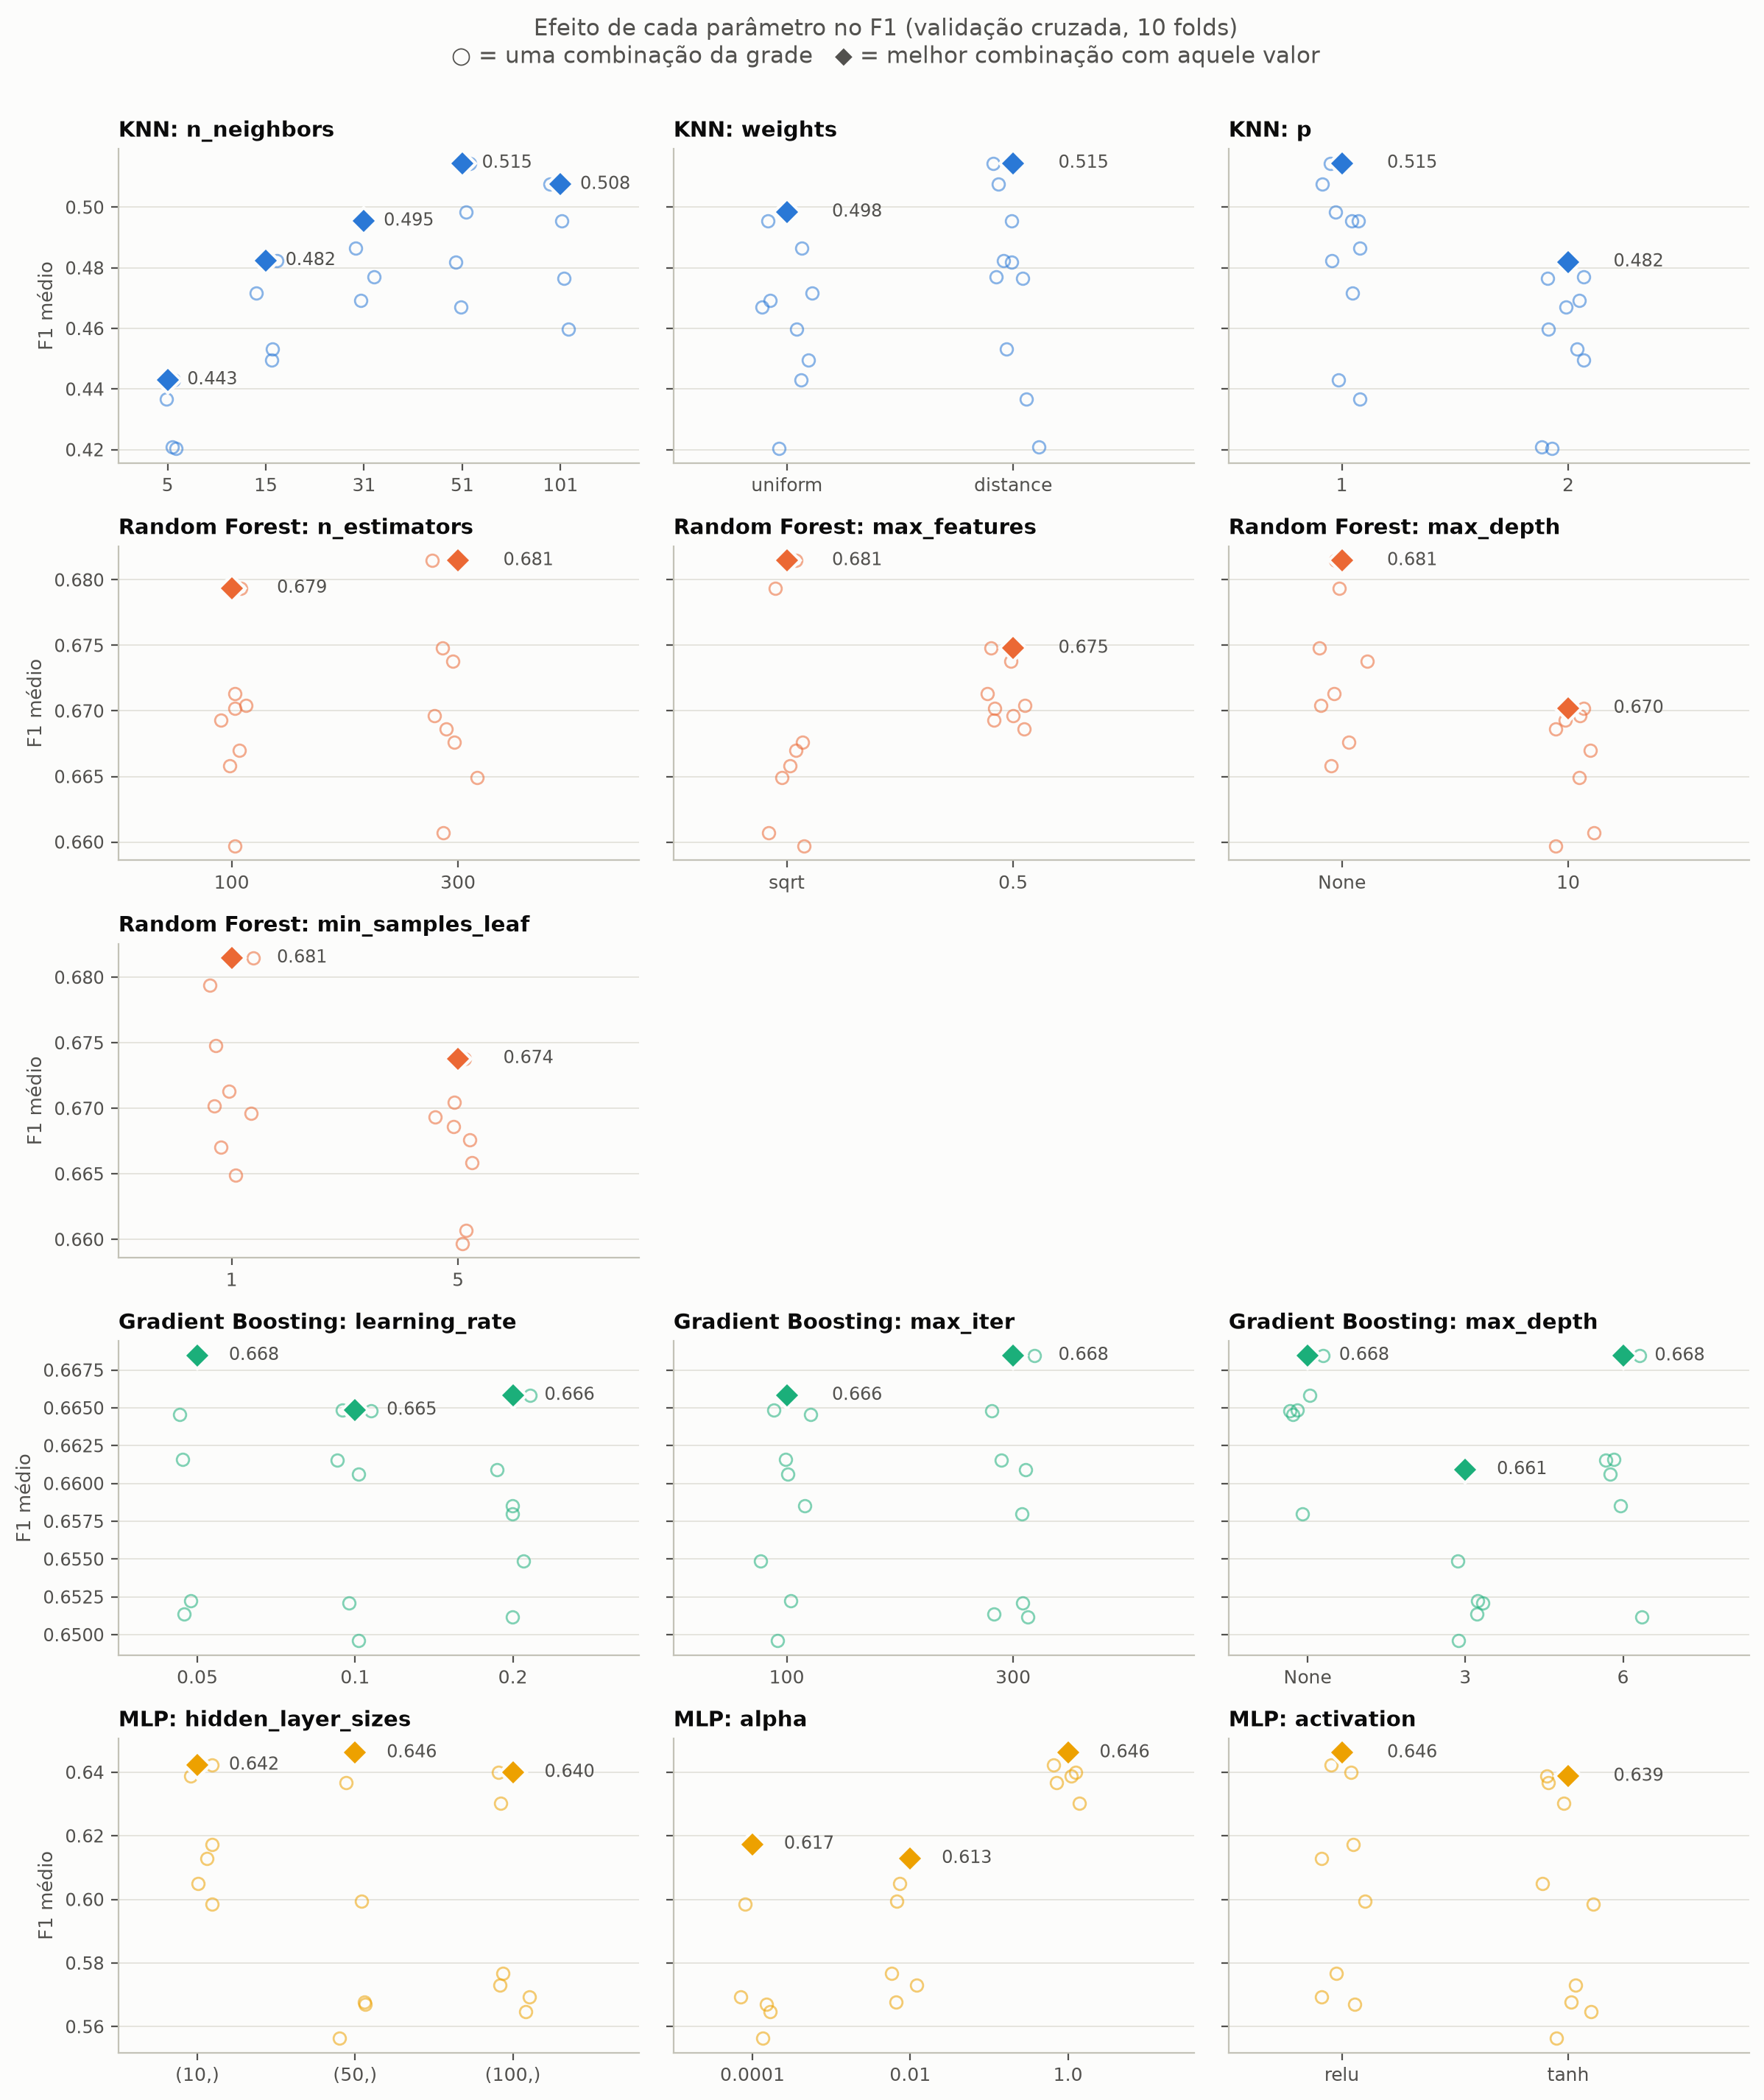
\includegraphics[width=\textwidth]{01_efeito_dos_parametros.png}
  \caption{Efeito de cada parâmetro no F1 médio da validação cruzada (10 folds). Cada círculo é uma combinação da
           grade, e o losango é a melhor combinação com aquele valor do parâmetro.}
  \label{fig:efeito}
\end{figure}

\begin{table}[H]
  \centering\small
  \caption{Sensibilidade de cada algoritmo aos parâmetros (F1 médio na validação cruzada).}
  \label{tab:sensibilidade}
  \begin{tabular}{lrrrrr}
    \toprule
    Algoritmo & Combinações & Pior F1 & Melhor F1 & Amplitude & Desvio padrão entre folds\\
    \midrule
    KNN & 20 & 0,420 & 0,515 & 0,094 & 0,021\\
    Random Forest & 16 & 0,660 & 0,681 & 0,022 & 0,030\\
    Gradient Boosting & 18 & 0,650 & 0,668 & 0,019 & 0,032\\
    MLP & 18 & 0,556 & 0,646 & 0,090 & 0,032\\
    \bottomrule
  \end{tabular}
\end{table}

No KNN e no MLP, a amplitude é cerca de três vezes o desvio padrão entre os folds: os parâmetros mudam o resultado de
fato. No MLP, a regularização foi decisiva: todas as combinações com $\alpha = 1$ ficaram entre 0,630 e 0,646 de F1,
enquanto as redes de 50 e 100 neurônios com $\alpha$ pequeno caíram para 0,556 a 0,599, porque decoram o treino. Com
regularização forte, o tamanho da camada e a função de ativação pesam pouco. No KNN, o F1 melhora com mais vizinhos
até $k = 51$ (de 0,443 com $k = 5$ para 0,515), a distância de Manhattan supera a euclidiana em todos os valores de
$k$ e o peso por distância ajuda um pouco. No Random Forest e no Gradient Boosting, as combinações ficam numa faixa
menor que o desvio padrão entre os folds, ou seja, esses algoritmos são pouco sensíveis aos parâmetros testados e os
valores padrão já funcionam bem.

A Tabela~\ref{tab:melhores} mostra a melhor parametrização de cada algoritmo, escolhida pelo maior F1 médio.

\begin{table}[H]
  \centering\footnotesize
  \setlength{\tabcolsep}{4pt}
  \caption{Melhor parametrização de cada algoritmo na validação cruzada (média $\pm$ desvio padrão dos 10 folds).}
  \label{tab:melhores}
  \begin{tabularx}{\textwidth}{@{}lYcccc@{}}
    \toprule
    Algoritmo & Melhor parametrização & F1 & PR-AUC & Precisão & Revocação\\
    \midrule
    KNN & $k = 51$, peso por distância, Manhattan ($p = 1$) & 0,515 $\pm$ 0,018 & 0,514 $\pm$ 0,030 & 0,392 & 0,749\\
    Random Forest & 300 árvores, \atr{max\_features} = sqrt, sem limite de profundidade, folha $\ge$ 1
      & 0,681 $\pm$ 0,036 & 0,738 $\pm$ 0,032 & 0,634 & 0,737\\
    Gradient Boosting & \atr{learning\_rate} = 0,05, 300 árvores, sem limite de profundidade
      & 0,668 $\pm$ 0,034 & 0,739 $\pm$ 0,034 & 0,602 & 0,753\\
    MLP & 50 neurônios, $\alpha = 1$, ReLU & 0,646 $\pm$ 0,031 & 0,700 $\pm$ 0,037 & 0,541 & 0,804\\
    \bottomrule
  \end{tabularx}
\end{table}

\subsection{Resultados no conjunto de teste}

A Tabela~\ref{tab:comparativa} é a tabela comparativa final, com as quatro medidas escolhidas calculadas no teste
para a melhor parametrização de cada algoritmo. A coluna ``F1 (val. cruzada)'' repete a estimativa da validação cruzada: em todos os
algoritmos, o F1 no teste ficou a no máximo 0,02 dela, o que confirma que a escolha dos parâmetros não foi
sobreajustada.

\begin{table}[H]
  \centering\small
  \caption{Tabela comparativa no conjunto de teste (2.441 sessões, 382 com compra), ordenada pelo F1. Em negrito, o
           melhor valor de cada medida.}
  \label{tab:comparativa}
  \begin{tabular}{lccccc}
    \toprule
    Algoritmo & F1 & PR-AUC & Precisão & Revocação & F1 (val. cruzada)\\
    \midrule
    Random Forest & \textbf{0,683} & \textbf{0,739} & \textbf{0,633} & 0,741 & 0,681\\
    Gradient Boosting & 0,666 & 0,727 & 0,588 & 0,767 & 0,668\\
    MLP & 0,655 & 0,710 & 0,549 & \textbf{0,814} & 0,646\\
    KNN & 0,535 & 0,555 & 0,403 & 0,796 & 0,515\\
    \bottomrule
  \end{tabular}
\end{table}

As matrizes de confusão (Figura~\ref{fig:matrizes} e Tabela~\ref{tab:matrizes}) mostram como cada algoritmo erra.

\begin{figure}[H]
  \centering
  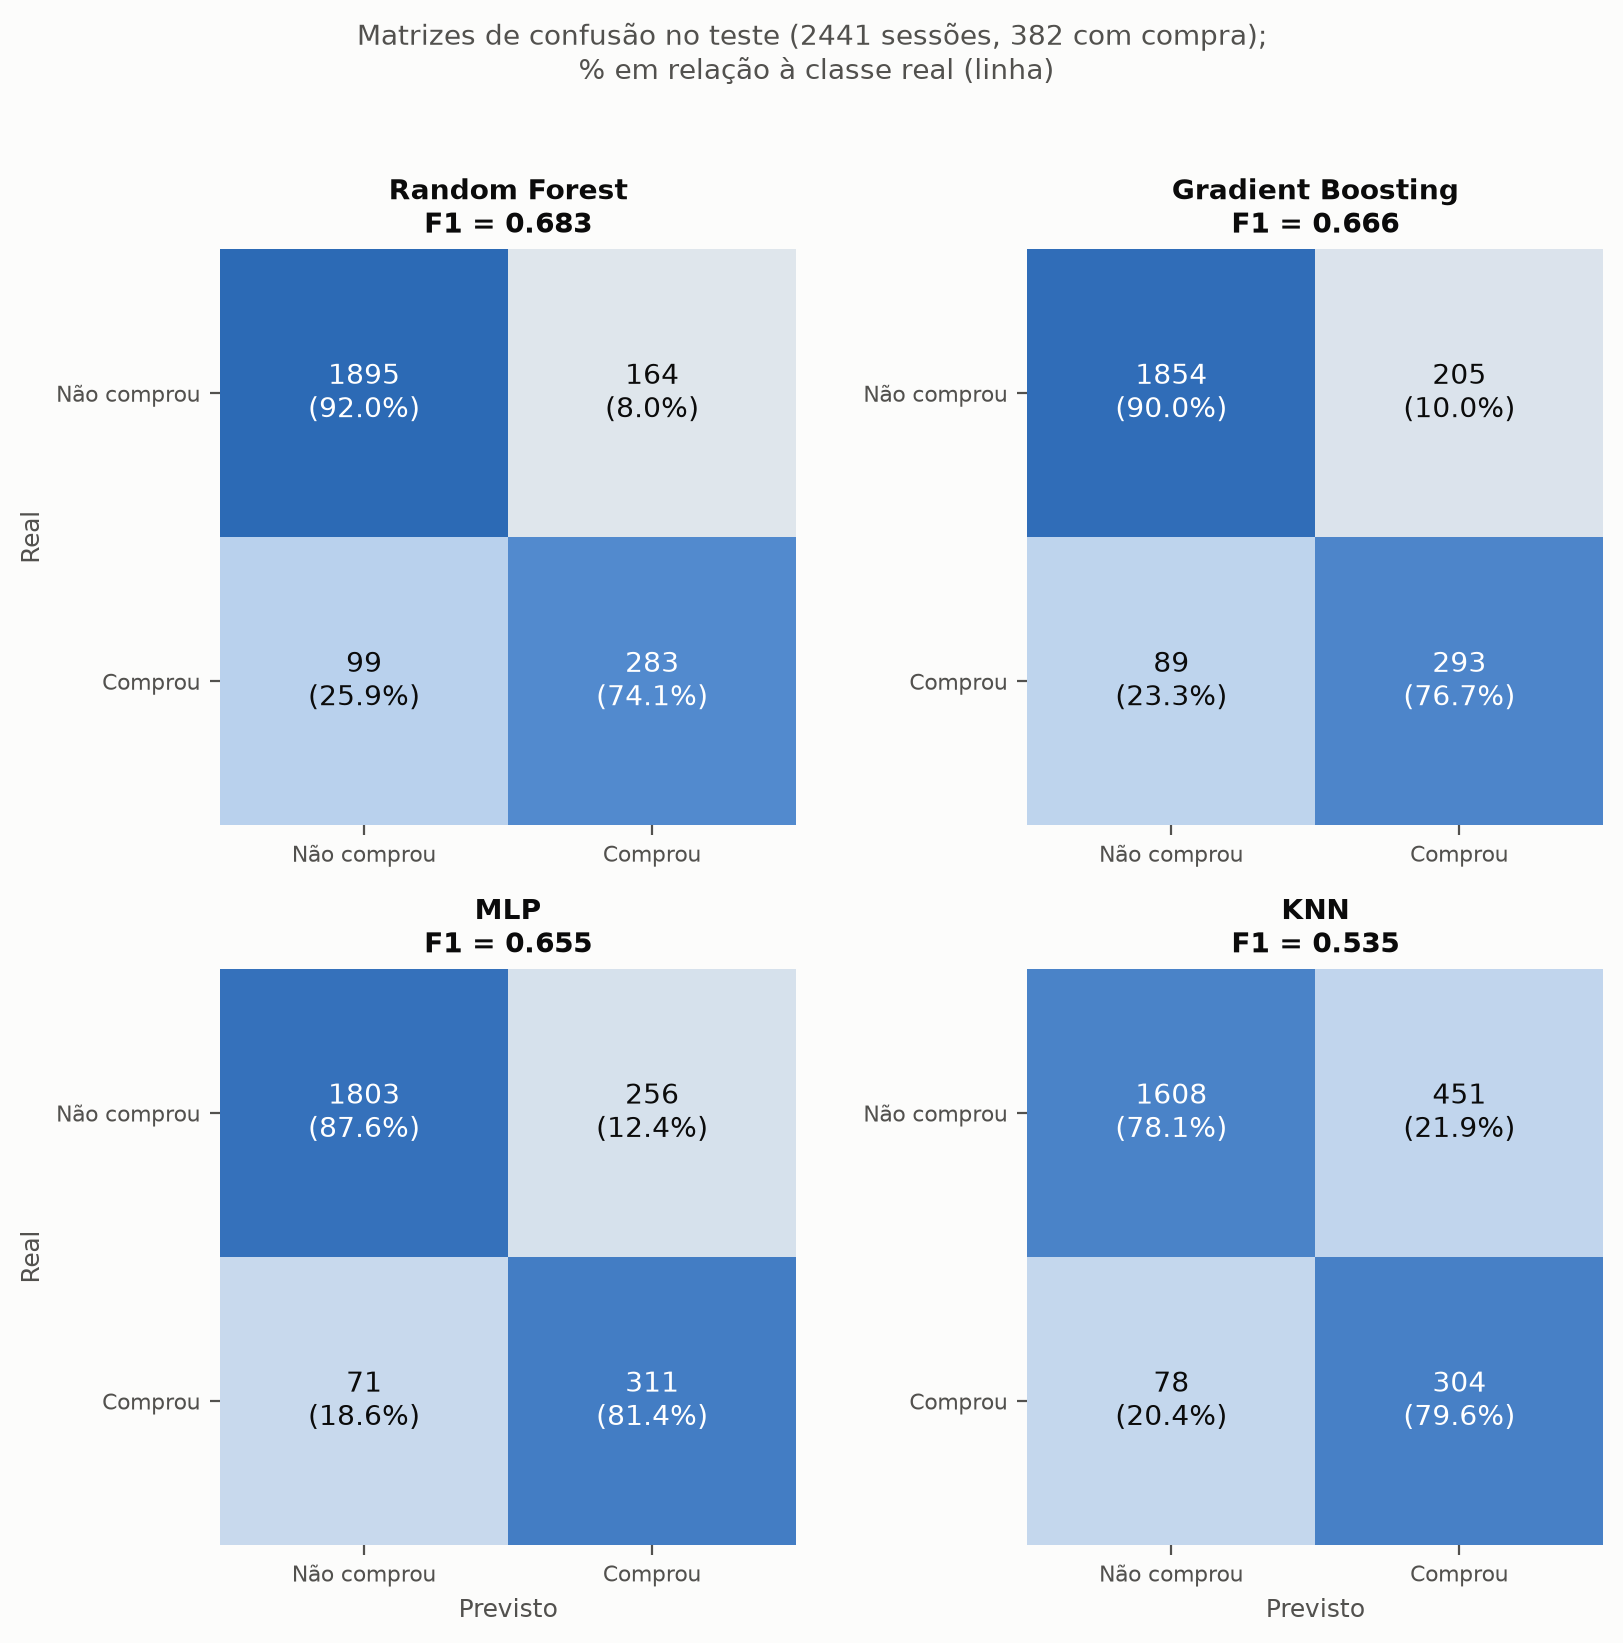
\includegraphics[width=0.82\textwidth]{02_matrizes_confusao_teste.png}
  \caption{Matrizes de confusão no conjunto de teste. As porcentagens são relativas à classe real (linha).}
  \label{fig:matrizes}
\end{figure}

\begin{table}[H]
  \centering\small
  \caption{Células das matrizes de confusão no teste.}
  \label{tab:matrizes}
  \begin{tabular}{lrrrr}
    \toprule
    Algoritmo & VN & \celula{FP\\(alarme falso)} & \celula{FN\\(comprador perdido)} & \celula{VP\\(comprador encontrado)}\\
    \midrule
    Random Forest & 1.895 & 164 & 99 & 283 (74,1\%)\\
    Gradient Boosting & 1.854 & 205 & 89 & 293 (76,7\%)\\
    MLP & 1.803 & 256 & 71 & 311 (81,4\%)\\
    KNN & 1.608 & 451 & 78 & 304 (79,6\%)\\
    \bottomrule
  \end{tabular}
\end{table}

A Figura~\ref{fig:curvas} mostra as curvas de precisão $\times$ revocação, cuja área é a PR-AUC. O ponto em cada curva
é o limiar padrão de 0,5, que gera as matrizes de confusão.

\begin{figure}[H]
  \centering
  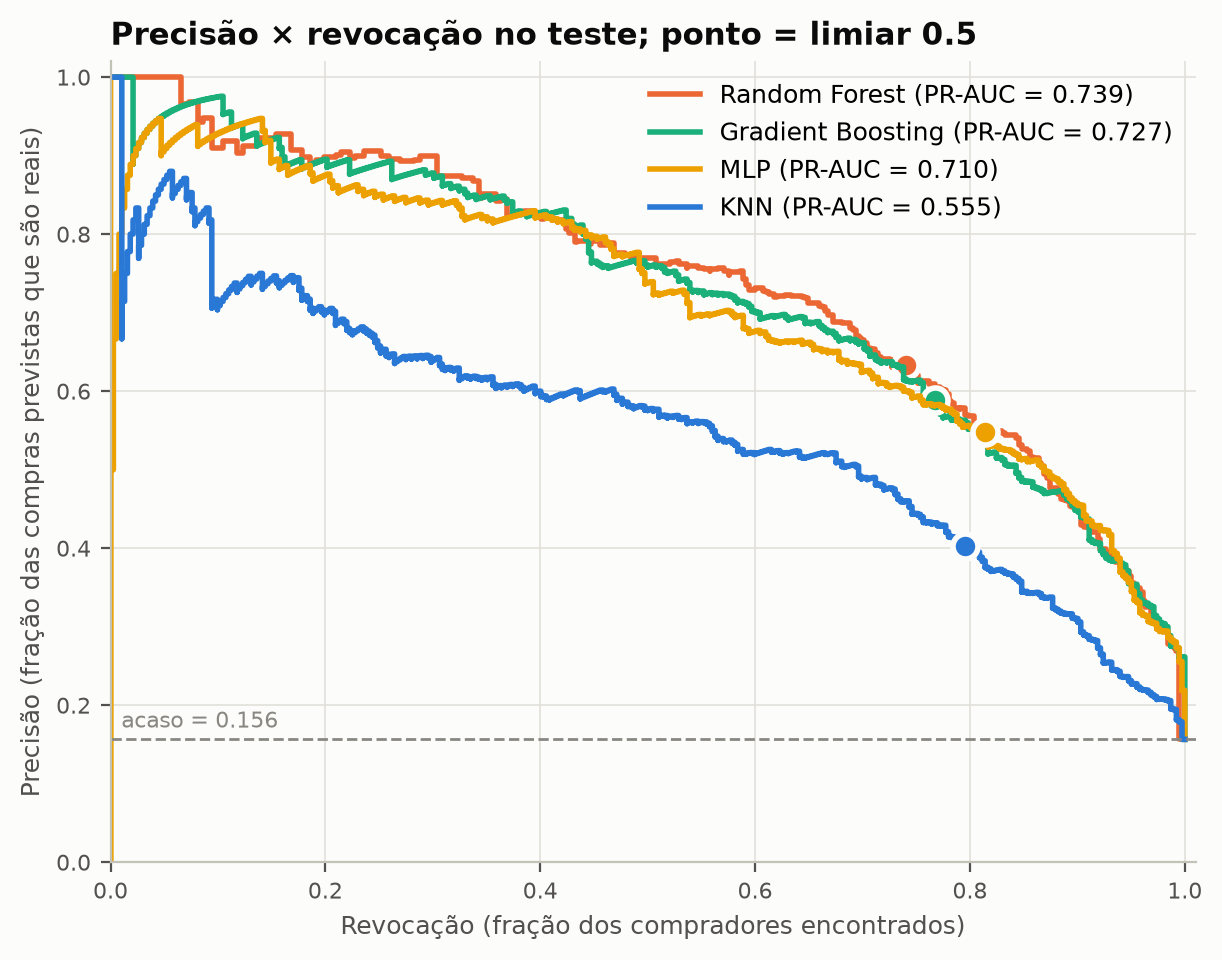
\includegraphics[width=0.72\textwidth]{03_curvas_precisao_revocacao_teste.png}
  \caption{Curvas de precisão $\times$ revocação no teste. O ponto marca o limiar de 0,5, e a linha tracejada é o
           desempenho de um classificador sem conhecimento.}
  \label{fig:curvas}
\end{figure}

\subsection{Discussão}

\textbf{Qual algoritmo apresentou o melhor desempenho? A resposta depende da medida?} O Random Forest foi o melhor
pelas duas medidas principais (F1 = 0,683 e PR-AUC = 0,739) e também pela precisão (0,633). A resposta, porém, depende
da medida: pela revocação, o melhor seria o MLP (0,814), porque ele prevê mais compras e, assim, encontra mais
compradores, à custa de mais alarmes falsos. É por isso que a decisão foi tomada pelo F1, que equilibra precisão e
revocação. Além disso, a diferença entre Random Forest e Gradient Boosting (0,017
de F1) é menor que o desvio padrão entre os folds, então os dois estão praticamente empatados; o KNN ficou claramente
atrás em todas as medidas, exceto a revocação.

\textbf{A alteração dos parâmetros modificou os resultados?} Sim, mas de forma muito diferente entre os algoritmos
(Tabela~\ref{tab:sensibilidade} e Figura~\ref{fig:efeito}). O KNN e o MLP mudaram bastante (amplitude de 0,094 e 0,090
de F1), com destaque para o número de vizinhos e a distância no KNN e para a regularização no MLP. O Random Forest e o
Gradient Boosting variaram menos que o desvio padrão entre os folds: são robustos à escolha dos parâmetros.

\textbf{Os algoritmos apresentaram comportamentos diferentes em relação aos erros?} Sim (Tabela~\ref{tab:matrizes}). O
Random Forest é o mais conservador: gera menos alarmes falsos (164), mas perde mais compradores (99). O MLP é o oposto:
perde menos compradores (71), mas gera 256 alarmes falsos. O Gradient Boosting fica entre os dois. O KNN encontra quase
tantos compradores quanto o MLP, mas à custa de 451 alarmes falsos, o que derruba sua precisão para 0,403.

\textbf{O desbalanceamento influenciou a avaliação?} Sim, de três formas. Primeiro, tornou a acurácia enganosa: 84,4\%
é atingido sem encontrar nenhum comprador, e a acurácia escolheria parametrizações que encontram menos compradores.
Segundo, deixou a ROC-AUC otimista: por ela, o KNN parece próximo dos demais (70\% do caminho até o modelo perfeito,
contra 86\% do Random Forest), mas pela PR-AUC a diferença aparece (44\% contra 70\%), porque a taxa de falsos positivos
é diluída pelos milhares de não-compradores. Terceiro,
o tratamento do desbalanceamento (sobreamostragem e \atr{class\_weight}) desloca os modelos a favor da classe
``comprou'': em todos os algoritmos a revocação ficou maior que a precisão, ou seja, os modelos preferem gerar alarmes
falsos a perder compradores.

\textbf{Quais características da base explicam as diferenças?} O atributo \atr{PageValues} domina o problema ($\rho =
0{,}63$ com a classe; 56,3\% das sessões com \atr{PageValues} $> 0$ compram, contra 3,9\% das demais). As árvores
exploram esse tipo de limiar diretamente, não são afetadas pela forte assimetria e pelos outliers e lidam bem com
atributos categóricos, o que explica o bom desempenho do Random Forest e do Gradient Boosting. Já o KNN depende de
distâncias, e o pré-processamento produziu 55 colunas, das quais 47 vêm do one-hot dos atributos categóricos: duas
sessões que diferem apenas no navegador ou no tipo de tráfego ficam tão distantes quanto duas com \atr{PageValues}
muito diferentes, e o atributo mais informativo perde peso. A vantagem da distância de Manhattan reforça essa
explicação, pois ela não reduz as diferenças pequenas dos atributos numéricos como a euclidiana (que as eleva ao
quadrado). O MLP precisou de regularização forte porque a base é pequena para uma rede neural (cerca de 9.800 sessões
de treino) e as redes maiores sem regularização decoraram o treino.

\textbf{Qual modelo recomendamos?} Recomendamos o \textbf{Random Forest} com 300 árvores e os demais parâmetros no
padrão. Ele teve o melhor resultado nas duas medidas escolhidas, é o mais preciso (menos alarmes falsos), foi estável
entre os folds e pouco sensível aos parâmetros, não exige normalização e permite inspecionar a importância dos
atributos. Numa aplicação real, a escolha final também depende do custo de cada erro: se perder um comprador custar
muito mais que um alarme falso (por exemplo, um cupom barato oferecido a quem não compraria), vale reduzir o limiar de
decisão do Random Forest, que pelas curvas da Figura~\ref{fig:curvas} atinge a mesma revocação do MLP com precisão
semelhante. O Gradient Boosting é uma alternativa praticamente equivalente.

% ============================================================================= V
\section{Conclusões}

\textbf{Principais aprendizados.}
\begin{itemize}
  \item Em problemas desbalanceados, a escolha da medida de avaliação muda as conclusões: a acurácia premiou o modelo
        que nunca encontra um comprador e teria escolhido parametrizações piores. O F1 e a PR-AUC, focados na classe
        minoritária, mostraram as diferenças reais.
  \item O pré-processamento precisa ser pensado para cada algoritmo: as árvores funcionaram bem quase sem
        transformações, enquanto o KNN e o MLP dependeram de escala, codificação e regularização.
  \item Ajustar as transformações e a sobreamostragem só nos dados de treino de cada fold, dentro de um pipeline, é
        essencial para que a avaliação não seja otimista por vazamento de informação.
  \item Testar vários parâmetros mostrou que alguns algoritmos (KNN e MLP) dependem muito da parametrização, enquanto
        outros (Random Forest e Gradient Boosting) já funcionam bem com os valores padrão.
\end{itemize}

\textbf{Limitações do experimento.}
\begin{itemize}
  \item O teste tem apenas 382 compradores; diferenças pequenas entre algoritmos (como entre Random Forest e Gradient
        Boosting) estão dentro da variação esperada entre amostras.
  \item A grade de parâmetros é limitada (72 combinações) e todos os modelos usaram o limiar de decisão padrão de
        0,5, sem ajuste ao custo de cada tipo de erro.
  \item No KNN, o one-hot dos atributos categóricos domina a distância, o que provavelmente subestima o potencial do
        algoritmo.
  \item A sobreamostragem aleatória apenas repete sessões, o que pode favorecer o sobreajuste; o par
        \atr{BounceRates} $\times$ \atr{ExitRates} (correlação de 0,91) foi mantido em todos os algoritmos.
  \item A base cobre um único site e um único ano, então os resultados podem não se generalizar para outras lojas ou
        períodos.
\end{itemize}

\textbf{Possíveis melhorias.}
\begin{itemize}
  \item Ajustar o limiar de decisão de acordo com o custo de cada erro para a loja.
  \item Melhorar o KNN reduzindo o peso dos atributos categóricos, usando apenas os atributos numéricos ou uma
        distância própria para dados mistos.
  \item Testar o SMOTENC no lugar da sobreamostragem aleatória e avaliar a remoção de \atr{BounceRates} ou
        \atr{ExitRates}.
  \item Ampliar a busca de parâmetros (busca aleatória ou bayesiana) e usar validação cruzada aninhada para estimar o
        desempenho com menos variância.
  \item Testar outras implementações de boosting (XGBoost, LightGBM) e analisar a importância dos atributos para
        interpretar as decisões do modelo recomendado.
\end{itemize}

% ============================================================================= VI
\section{Referências}

\begin{list}{}{\setlength{\leftmargin}{1.2em}\setlength{\itemindent}{-1.2em}\setlength{\itemsep}{4pt}}
  \item BREIMAN, L. Random forests. \textit{Machine Learning}, v. 45, n. 1, p. 5--32, 2001.
  \item FRIEDMAN, J. H. Greedy function approximation: a gradient boosting machine. \textit{The Annals of
        Statistics}, v. 29, n. 5, p. 1189--1232, 2001.
  \item HARRIS, C. R. et al. Array programming with NumPy. \textit{Nature}, v. 585, p. 357--362, 2020.
  \item HUNTER, J. D. Matplotlib: a 2D graphics environment. \textit{Computing in Science \& Engineering}, v. 9, n. 3,
        p. 90--95, 2007.
  \item KE, G. et al. LightGBM: a highly efficient gradient boosting decision tree. In: \textit{Advances in Neural
        Information Processing Systems 30 (NIPS 2017)}, 2017.
  \item KINGMA, D. P.; BA, J. Adam: a method for stochastic optimization. In: \textit{International Conference on
        Learning Representations (ICLR)}, 2015.
  \item LEMAÎTRE, G.; NOGUEIRA, F.; ARIDAS, C. K. Imbalanced-learn: a Python toolbox to tackle the curse of imbalanced
        datasets in machine learning. \textit{Journal of Machine Learning Research}, v. 18, n. 17, p. 1--5, 2017.
  \item MCKINNEY, W. Data structures for statistical computing in Python. In: \textit{Proceedings of the 9th Python in
        Science Conference}, p. 56--61, 2010.
  \item PEDREGOSA, F. et al. Scikit-learn: machine learning in Python. \textit{Journal of Machine Learning Research},
        v. 12, p. 2825--2830, 2011.
  \item RUMELHART, D. E.; HINTON, G. E.; WILLIAMS, R. J. Learning representations by back-propagating errors.
        \textit{Nature}, v. 323, p. 533--536, 1986.
  \item SAITO, T.; REHMSMEIER, M. The precision-recall plot is more informative than the ROC plot when evaluating
        binary classifiers on imbalanced datasets. \textit{PLoS ONE}, v. 10, n. 3, e0118432, 2015.
  \item SAKAR, C. O.; POLAT, S. O.; KATIRCIOGLU, M.; KASTRO, Y. Real-time prediction of online shoppers' purchasing
        intention using multilayer perceptron and LSTM recurrent neural networks. \textit{Neural Computing and
        Applications}, v. 31, p. 6893--6908, 2019.
  \item SAKAR, C. O.; KASTRO, Y. Online Shoppers Purchasing Intention Dataset. UCI Machine Learning Repository, 2018.
        Disponível em: \url{https://archive.ics.uci.edu/dataset/468/online+shoppers+purchasing+intention+dataset}.
  \item Ferramentas: Python 3.13 (\url{https://www.python.org}), Jupyter (\url{https://jupyter.org}) e uv
        (\url{https://docs.astral.sh/uv}).
\end{list}

\end{document}
